\documentclass[]{article}
\usepackage{etex}
\usepackage[margin = 1.5in]{geometry}
\setlength{\parindent}{0in}
\usepackage{amsmath}
\usepackage{amsfonts}
\usepackage{amssymb}
\usepackage{amsthm}
\usepackage{mathtools}
\usepackage{pgfplots}
\usepackage[lined]{algorithm2e}
\usepackage{hyperref}
\usepackage{qtree}
\usepackage{xytree}
\usepackage{float}
\usepackage{cleveref}
\usepackage[T1]{fontenc}
\usepackage{ae,aecompl}

\theoremstyle{definition}
\newtheorem*{defn}{Definition}
\newtheorem{ex}{Example}[section]
\newtheorem*{theorem}{Theorem}

\setlength{\marginparwidth}{1.5in}
\setlength{\algomargin}{0.75em}

\DeclarePairedDelimiter{\set}{\lbrace}{\rbrace}

\definecolor{darkish-blue}{RGB}{25,103,185}

\usepackage{hyperref}
\hypersetup{
    colorlinks,
    citecolor=darkish-blue,
    filecolor=darkish-blue,
    linkcolor=darkish-blue,
    urlcolor=darkish-blue
}
\newcommand{\lecture}[1]{\marginpar{{\footnotesize $\leftarrow$ \underline{#1}}}}

\stepcounter{footnote} % because daggers are cool

\begin{document}
	\let\ref\Cref

	\title{\bf{CS 240: Data Structures and Data Management}}
	\date{Winter 2013, University of Waterloo \\ \center Notes written from Alejandro L\'opez-Ortiz's lectures.}
	\author{Chris Thomson\thanks{See \href{https://github.com/christhomson/lecture-notes}{github.com/christhomson/lecture-notes}.
	\ifdefined\sha % Also, \commitDate and \commitTime should be defined.
		Last modified: \commitDateTime{} ({\href{https://github.com/christhomson/lecture-notes/commit/\sha}{\sha}}).
	\fi}}
	\maketitle
	\newpage
	\tableofcontents
	\newpage

	\section{Introduction \& Code Optimization} \lecture{January 8, 2013}
		\subsection{Course Structure}
			The grading scheme is 50\% final, 25\% midterm, and 25\% assignments. There are five assignments, usually due on Wednesday mornings at 9:30 am. There are several textbooks for the course, all of which are optional but recommended. The textbooks cover roughly 80\% of the course content. There are also \href{https://www.student.cs.uwaterloo.ca/~cs240/w13/lectures.phtml}{some course notes available online} from previous terms, however the lectures will not necessarily follow those notes strictly.
			\\ \\
			See the \href{https://www.student.cs.uwaterloo.ca/~cs240/w13/info.phtml}{course syllabus} for more information.

		\subsection{CS as the Science of Information}
			So far in our undergraduate careers, computer science has meant programming. However, programming is only a subset of computer science. Computer science is the \textbf{science of information}.
			\\ \\
			What do we want to do with information? We want to:
			\begin{itemize}
				\item \textbf{Process it}. Programs $\equiv$ algorithms.
				\item \textbf{Store it}. We want to encode it. This also leads to information theory. Storing information involves data structures, databases, (file) systems, etc., all of which are searchable in some way.
				\item \textbf{Transmit it}. We want to transmit information over networks. This process involves coding theory.
				\item \textbf{Search it}. First, we have to structure it with data structures and/or SQL databases. Information retrieval is the process of searching for textual information instead of numerical information.
				\item \textbf{Mine it}. This involves artificial intelligence and machine learning.
				\item \textbf{Display it}. Information needs to be displayed using computer graphics (CG) and user interfaces (UI, partially related to psychology).
				\item \textbf{Secure it}. Encryption and cryptography are important. Information should also be stored redundantly to prevent harm from catastrophic events.
			\end{itemize}

		\subsection{Objectives of the Course}
			\begin{itemize}
				\begin{item}
					\textbf{Study efficient methods of storing, accessing, and performing operations on \underline{large} collections of data.} \\ \\
					``Large" is subjective -- your data needs to be large enough to justify the additional mental complexity. \\ \\
					Typical operations:
					\begin{itemize}
						\item Insert new item.
						\item ``Deleting" data (flagging data as ``deleted," not actually deleting the data).
						\item Searching for data.
						\item Sorting the data. \\
					\end{itemize}

					Examples of ``large data":
					\begin{itemize}
						\item The web.
						\item Facebook data.
						\item DNA data.
						\item LHC (Large Hadron Collider) measurements (terabytes per day).
						\item All the music from iTunes, for finding duplicate songs, etc.
					\end{itemize}
				\end{item}

				\begin{item}
					\textbf{There is a strong emphasis on mathematical analysis.} \\ \\
					The performance of algorithms will be analyzed using order notation.
				\end{item}

				\begin{item}
					\textbf{The course will involve abstract data types (objects) and data structures.} \\ \\
					We will see examples that have to do with:
					\begin{itemize}
						\item Databases.
						\item Geographic databases.
						\item Text searching.
						\item Text compression.
						\item Web searching.
					\end{itemize}
				\end{item}
			\end{itemize}

		\subsection{Code Optimization \& Measuring Performance}
			Richard Feynman was in charge of the computer group on the Manhattan Project. He made his code run 10x faster.
			\\ \\
			The initial method to measure performance was to use a \textbf{wall clock}. Initial studies looked like this:

			\begin{center}
				\begin{tabular}{|c|c|c|}
					\hline
					Data size & A & B \\ \hline
					3 & 1 & 3 \\
					5 & 2 & 9 \\
					10 & 4 & 10 \\
					20 & 16 & 11 \\ \hline
				\end{tabular}
			\end{center}

			However, computers were getting better, so we couldn't use wall clocks anymore. Results were not robust enough due to the quick progression of performance increases in terms of computing power. Moreover, because of the differences in architecture, the same program may have a different execution time on two different computer models.
			\\ \\
			\underline{Idea}: rather than comparing algorithms using seconds, we should compare algorithms using the number of operations required for the algorithm to run.

			\begin{itemize}
				\item Express algorithm using pseudocode.
				\item Count the number of primitive operations.
				\item Plot the number of operations vs. the input size. \\
			\end{itemize}

			\begin{figure}
				\centering
				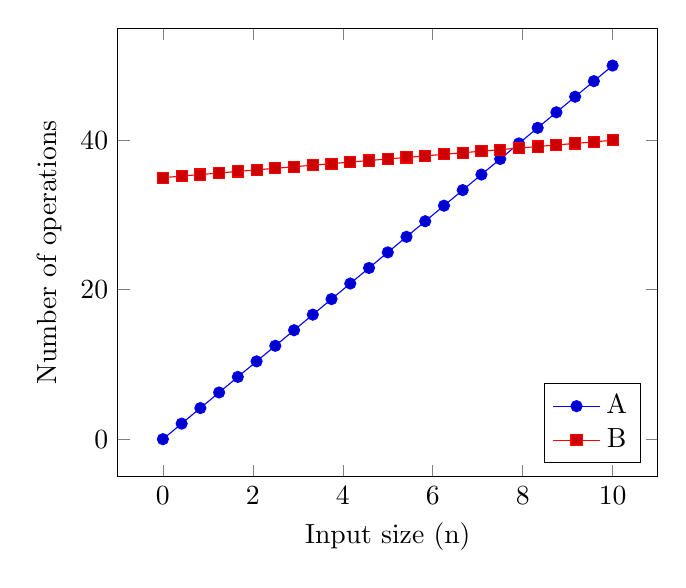
\begin{tikzpicture}[domain=0:10]
					\begin{axis}[
						xlabel = Input size (n),
						ylabel = Number of operations,
						legend entries = {A,B},
						legend pos = south east]
						\addplot{5*x};
						\addplot{0.5*x+35};
					\end{axis}
				\end{tikzpicture}
				\caption{A comparison of two algorithms $A$ and $B$.}
			\end{figure}

			Note that $A$ and $B$ are plotted as continuous functions, however they are not actually continuous -- we join all of the points for readability purposes only.
			\\ \\
			In the long run, you may want to use algorithm $B$ even if algorithm $A$ is better in some cases, because the benefits of $A$ will be short lived as $n$ grows.
			\\ \\
			Hence, comparing the programs has been transformed into comparing functions. We use order notation to measure the long-term growth of functions, allowing us to choose the smaller function, which corresponds to the faster algorithm.

	\section{Order Notation} \lecture{January 10, 2013}
		The time for algorithm $A$ on input of size $n$ is:

		\begin{align*}
			\underbrace{2n \log n}_\text{sort} + \underbrace{1.5n^3}_\text{mult} + \underbrace{22n^2 - 3n}_\text{additions} + \underbrace{7}_\text{setup}
		\end{align*}

		On a different machine, the same algorithm $A$ may be $2n \log n + 9n^3 + 10n^2 - 3n + 7$. These give a \textbf{false sense of precision}. These specifics can also be quite costly to determine. In the 1960s, Don Knuth proposed \textbf{order notation} as a way to analyze the general quality of algorithms in an accurate, cost- and time-efficient way by ignoring precise runtimes.

		\subsection{Formal Definitions}
			Order notation represents algorithms as functions. We say a function $f(n)$ relates to a certain order $g(n)$ using different notation depending on which relation we're interested in.
			\begin{center}
				\begin{tabular}{|c|c|}
					\hline
					 Relation & Functions \\ \hline
					 $3 \le 7$ & $f(n) = O(g(n))$ \\
					 $8 \ge 7$ & $f(n) = \Omega(g(n))$ \\
					 $7 = 7$ & $f(n) = \Theta(g(n))$ \\
					 $3 < 7$ & $f(n) = o(g(n))$ \\
					 $7 > 3$ & $f(n) = \omega(g(n))$ \\ \hline
				\end{tabular}
			\end{center}

			Here's an easy way to remember the correspondence between a relation and its order notation symbol: the greedy operators, $\le$ and $\ge$, are uppercase letters $O$ and $\Omega$. The less greedy operators, $<$ and $>$, are the same letters but in lowercase ($o$ and $\omega$). \\

			Order notation only cares about the long run. An algorithm can violate the relation early -- we're interested in its asymptotic behavior.

			\begin{defn}[$\le$]
				$f(n) = O(g(n))$ if there exist constants $c > 0, n_0 > 0$ such that $f(n) \le c \cdot g(n)$ for all $n \ge n_0$.
			\end{defn}

			\begin{defn}[$\ge$]
				$f(n) = \Omega(g(n))$ if there exist constants $c > 0, n_0 > 0$ such that $f(n) \ge c \cdot g(n)$ for all $n \ge n_0$.
			\end{defn}

			\begin{defn}[$=$]
				$f(n) = \Theta(g(n))$ if there exists constants $c_1, c_2 > 0$ such that $c_1 \cdot g(n) \le f(n) \le c_2 \cdot g(n)$.
			\end{defn}

			The equality relation is effectively sandwiching the algorithm $f(n)$ between two other functions (the squeeze theorem). If it's possible to sandwich the algorithm between two multiples of the same $g(n)$, then $f(x)$ is said to be equal to the order $g(n)$.

			\begin{defn}[$<$]
				$f(n) = o(g(n))$ if for all $c > 0$ there exists constant $n_0 > 0$ such that $f(n) < c \cdot g(n)$ for all $n \ge n_0$.
			\end{defn}

			\begin{defn}[$>$]
				$f(n) = \omega(g(n))$ if for all $c > 0$ there exists constant $n_0 > 0$ such that $f(n) > c \cdot g(n)$ for all $n \ge n_0$.
			\end{defn}

		\subsection{Order Notation Examples}
			\begin{ex}
				$2n^2 + 3n + 11 = O(n^2)$
				\\ \\
				We need to show that there exists constants $c > 0$ and $n_0 > 0$ such that $2n^2 + 3n + 11 \le cn^2$ for all $n \ge n_0$.
				\\ \\
				Let $c = 3$. Simplifying gets us $3n + 11 \le n^2$. This holds for $n_0 = 1000$, for instance.
			\end{ex}

			\begin{ex}
				$2n^2 + 3n + 11 1 = \Theta(n^2)$
				\\ \\
				In order to show equality ($\Theta$), we need to show both the $\le$ and $\ge$ cases. In the previous example, the $\le$ case was shown. For the $\ge$ case, we need to show $n^2 \le c \cdot (2n^2 + 3n + 11)$.
				\\ \\
				Let $c = 1$. Simplifying gets us $n^2 \le 2n^2 + 3n + 11$, which gives us $0 \le n^2 + 3n + 11$. This holds for $n_0 = 0$.
			\end{ex}

			\begin{ex}
				$2010n^2 + 1388 = o(n^3)$
				\\ \\
				We must show that for all $c > 0$, there exists $n_0 > 0$ such that $2010n^2 + 1388 \le c \cdot n^3$ for all $n \ge n_0$.

				\begin{align*}
					\frac{2010n^2+1388}{n^3} \stackrel{?}{\le} \frac{c \cdot n^3}{n^3} \implies \frac{2010}{n} + \frac{1388}{n^3} \stackrel{?}{\le} c
				\end{align*}

				There is a \textbf{trick to prove f(n) = o(g(n))}: show that $\lim_{n \to \infty}{}\frac{f(n)}{g(n)} = 0$.
			\end{ex}

		\subsection{A note about the use of =}
			\begin{align*}
				\underbrace{2n^2}_\text{specific function} \in \underbrace{O(n^2))}_\text{set of functions}
			\end{align*}

			The use of the equality operator ($=$) in order notation is not the same as in most other areas of mathematics, since a single element of a set cannot strictly be equal to the set itself (even $a \ne \set{a}$). The $=$ in order notation is not a true equality -- it's just notation. The $\in$ operator is semantically more correct.

		\subsection{Performance of Algorithms}
			We have made some progression in how we determine the performance of algorithms.
			\begin{itemize}
				\item Comparing single runs.
				\item Comparing measured curves (multiple runs).
				\item Produce analytical expressions for the curves.
				\item Simplify using order notation.
			\end{itemize}

			Let's say we have the problem of integrating a mathematical function. Our program numerically integrates the function, and we're trying to analyze the algorithm behind that process. The timing would vary depending on the mathematical function and preciseness required.
			\\ \\
			If we conduct multiple runs of our algorithm, we'll get different times. Plotting all of the results (time vs. input size) will result in data that is not a function, because the data fails the vertical line test, since for a given input size we have multiple times.
			\\ \\
			We need to decide on a convention for these cases where we have multiple time values. In this course, we'll usually look at the worst case, however in some situations examining the best or average cases could be useful.
			\\ \\
			Finding the average case is hard. To produce an appropriate average, we need an input distribution.
	\section{Formalism} \lecture{January 15, 2013}
		\begin{defn}
			A \textbf{problem} is a collection of questions and (correct) answer pairs.
		\end{defn}

		\begin{ex}
			Informally, the problem is ``multiplying two numbers.'' More formally, the problem could be represented as: (2 x 3, 6), (3 x 4, 12), (1 x 5, 5), etc.
		\end{ex}

		\begin{defn}
			An \textbf{instance} of a problem is a specific question and answer pair, (Q, A).
		\end{defn}

		\begin{defn}
			The \textbf{input} of a problem is the question. Example: 3 x 4.
		\end{defn}

		\begin{defn}
			The \textbf{output} is the only correct answer. Note: there is only one correct answer under this definition. ``Multiple'' correct answers can always be reduced to some canonical form that represents the one correct answer.
		\end{defn}

		\begin{defn}
			An \textbf{algorithm} is a mechanical method to produce the answer to a given question of a problem.
		\end{defn}

		\begin{defn}
			The \textbf{size of the input} is the number of bits, characters, or elements in the question. This definition will vary depending on what's most appropriate for the given question.
		\end{defn}

		Long division in elementary school was the first time a problem's complexity was directly related to the input size. That's not always the case, however.

		\begin{defn}
			We say an algorithm \textbf{solves} a problem if for every question $Q$ it produces the correct answer, $A$.
		\end{defn}

		\begin{defn}
			A \textbf{program} is an implementation of an algorithm using a specified computer language.
		\end{defn}

		\begin{ex}
			We want to sort $n$ numbers. One instance of this problem $Q$ is:
			\begin{align*}
				(\underbrace{(5, 1, 3, 2, 4)}_\text{Q}, \underbrace{(1, 2, 3, 4, 5)}_\text{A})
			\end{align*}

			For a problem in this form, we'll say the size of $Q$ is $|I| = 5$. Why? Counting the number of elements is the most logical definition in this case.
		\end{ex}

		This course emphasizes algorithms rather than programs. We're computer scientists, so we care about the algorithm and the speed/efficiency of that algorithm.
		\\ \\
		A problem $\Pi$ can have several correct algorithms that solve it. Our goal is to find efficient solutions to $\Pi$. How do we do that?
		\begin{enumerate}
			\item \textbf{Algorithm design}. Find a solution(s) to $\Pi$.
			\item \textbf{Algorithm analysis}. Assess the correctness and efficiency of the algorithm.
		\end{enumerate}

		In this course, we're mostly interested in algorithm analysis. Algorithm design will be covered in more detail in CS 341.

		\subsection{Timing Functions}
			A timing function is a function $T_{\mathcal{A}}$ such that:
			\begin{align*}
				T_{\mathcal{A}}: \set{Q } \to \mathbb{R}^{+}
			\end{align*}
			where $\mathbb{R}^{+}$ is the set of positive real numbers.
			\\ \\
			$T_{\mathcal{A}}(Q)$ is the time taken by algorithm $\mathcal{A}$ to compute the answer to $Q$.
			\\ \\
			We also want to define a general timing function for a particular problem, regardless of algorithm:
			\begin{align*}
				T(n) &= max \set{T_{ \mathcal{A}}(Q) } \\
				T_{avg}(n) &= avg \set{T_{\mathcal{A}}(Q) } \\
				T_{min}(n) &= min \set{T_{\mathcal{A}}(Q) } \\
				\vdots&
			\end{align*}

			If we had two solutions (algorithms) $T_A(n)$ and $T_B(n)$, we could use order notation to compare the quality of $A$ and $B$.
			\\ \\
			Note that some problem instances are easier than others to solve, even with the same input size. Most people find it easier to multiply $0 \times 7$ than $8 \times 7$, for instance, despite those two problems having the same input size.
	\section{Analysis of Algorithms}
		In order to analyze an algorithm, we count the number of \underline{basic} operations that the algorithm performs.
		\begin{ex}
			Let's say our algorithm is to compute $x^2 + 4x$ and assign it to a variable called \verb+result+. That involves seven basic operations:
			\begin{enumerate}
				\item Read $x$ from memory.
				\item Compute $x \cdot x$.
				\item Assign the result of $x \cdot x$ to a variable, \verb+pr1+.
				\item Compute $4 \cdot x$.
				\item Assign the result of $4 \cdot x$ to a variable, \verb+pr2+.
				\item Compute \verb+pr1+ + \verb+pr2+.
				\item Assign the result of \verb+pr1+ + \verb+pr2+ to a variable, \verb+result+.
			\end{enumerate}
		\end{ex}

		The number of operations remains the same across machines, but the actual running time of an algorithm will differ from machine to machine (which one of the reasons why we use order notation).
		\\ \\
		We only count the number of \underline{basic} operations. There are various definitions of what a ``basic'' operation actually is (especially with regards to variable assignments), but these are some common operations that are considered to be basic:
		\begin{itemize}
			\item Add numbers of reasonable size (numbers that can be added primitively).
			\item Multiply numbers of reasonable size (numbers that can multiplied primitively).
			\item Access an index in an array.
			\item Store a value in memory (variable assignments).
			\item Read a value from memory.
		\end{itemize}
		Be careful. Some languages disguise complexity well. Just because the syntax is simple doesn't necessarily mean it's a basic operation, and doesn't guarantee that the operation runs in constant time.

		\subsection{Techniques for Algorithm Analysis}
			\begin{itemize}
				\item Straight line programs (no loops). Simply tally up the basic operation count.
				\item Loops (\verb+for+/\verb+while+). You need to add the number of operations for each pass on the body of the loop.
			\end{itemize}

			\begin{ex}
				Analyze the following algorithm. \\
				\begin{algorithm}[H]
					\For{i = a to b}{
						< straight line program > $T_L$
					}
				\end{algorithm}
				This program will run with $\sum_{i = a}^{b} T_L(i)$ operations.
			\end{ex}

			Whenever you have a loop in your algorithm, you should expect to get a summation in your timing function.
			\begin{ex}
				Analyze the following algorithm. \\
				\begin{algorithm}[H]
					\For{x = 0 to 10}{
						pr1 = x * x\;
						pr2 = 4 * x\;
						result = pr1 + pr2\;
						print result\;
					}
				\end{algorithm}

				This program will run with $\sum_{i = 0}^{10} 4 = 44$ operations (depending on your definition of ``basic'' operations).
			\end{ex}

			Operations like addition and multiplication are primitive for numbers of a reasonable size. Once numbers get large enough to exceed certain limits, we have to resort to some trickery to perform those operations, which adds additional complexity, making them no longer ``basic'' operations.
			\\ \\
			We can be a bit sloppy and use the worst case, then say the actual algorithm is $\le$ to what we calculated.
			\begin{ex}
				Analyze the following algorithm. Test 1 ($n$). \\
				\begin{algorithm}[H]
					sum = 0\;
					\For{i = 1 to n}{
						sum = sum + i
					}
					\Return sum
				\end{algorithm}
				This program will run with $1 + (\sum_{i = 1}^n 1) + 1 = 2 + n = \Theta(n)$ operations.
			\end{ex}

			\begin{ex}
				Analyze the following algorithm. \\
				\begin{algorithm}[H]
					sum = 0\;
					\For{i = 1 to n}{
						\For{j = 1 to i}{
							$sum = sum + (i - j)^2$\;
							$sum = sum^2$\;
						}
					}
					\Return sum

				\end{algorithm}

				This program will run with time:
				\begin{align*}
					& 1 + \sum_{i = 1}^{n} \bigg[ \sum_{j = 1}^{i} 4 \bigg] + 1 \\
					&= 2 + \sum_{i = 1}^{n} 4i \\
					&= 2 + 4 \sum_{i = 1}^{n} i \\
					&= 2 + 4 \cdot \frac{n(n+1)}{2} \text{ (Gauss)} \\
					&= 2 + 2n^2 + 2n \\
					&= \Theta(n^2)
				\end{align*}

				We can be pessimistic, assume worst-case scenario, and say that it runs with time:
				\begin{align*}
					&2 + \sum_{i = 1}^{n} n \\
					&= O(n^2)
				\end{align*}

				Note that $O(n^2)$ is a less precise result than $\Theta(n^2)$, but in some cases that's good enough.
			\end{ex}

			Order notation helps make algorithm analysis easier by allowing us to throw away any specific constants, as long as the order remains untouched. The entire analysis process happens within the context of order notation, so you can just start dropping constants immediately.
			\\ \\
			Keep in mind, it is possible to create a bad over-estimation. You have to be smart about it.

			\begin{ex}
				Analyze the following algorithm. Test 2 (A, n). \\
				\begin{algorithm}[H]
					max = 0\;
					\For{i = 1 to n}{
						\For{j = 1 to n}{
							sum = 0\;
							\For{k = i to j}{
								sum = A[k] + sum\;
								\If{sum > max}{
									max = sum\;
								}
							}
						}
					}
					\Return max
				\end{algorithm}

				This is the \textbf{maximum subsequence problem}. The input is an array of integers $A[1\dots n]$, and the output is the consecutive run with the largest sum.
				\\ \\
				Sample sequence:
				\begin{tabular}{|c|c|c|c|c|c|c|}
					\hline 2 & -4 & 1 & 3 & -2 & 8 & -1 \\ \hline
				\end{tabular}
				\\ \\
				The running time of this program is $max \set{\sum_{i = 1}^{j} A[k] \big| 1 \le i \le j \le n}$.
			\end{ex}

			\begin{ex}
				\lecture{January 17, 2013}
				Analyze the following algorithm.
				\begin{algorithm}
					\For{i = 1 to n}{
						\For($L_1[i]$){j = 1 to i}{
							\For($L_2[i, j]$){k = 1 to j}{
								x = x + 1
							}
						}
					}
				\end{algorithm}

				\begin{align*}
					\sum_{i = 1}^{n} L_1(i) &= \sum_{i = 1}^{n} \bigg[\sum_{j = 1}^{i} L_2(i, j)\bigg] \\
					&= \sum_{i = 1}^{n} \bigg[ \sum_{j = 1}^{i} \bigg[ \sum_{k = 1}^{j} \Theta(1) \bigg] \bigg] \\
					&= \sum_{i = 1}^{n} \sum_{j = 1}^{i} \sum_{k = 1}^{j} 1 \\
					&= \sum_{i = 1}^{n} \sum_{j = 1}^{i} j \\
					&= \sum_{i = 1}^{n} \frac{i(i+1)}{2} \\
					&= \frac{1}{2} \sum_{i = 1}^{n}(i^2 + i) \\
					&= \frac{1}{2} \bigg[ \sum_{i = 1}^{n} i^2 + \sum_{i = 1}^{n} i \bigg] \\
					&= \frac{1}{2} \bigg[ \frac{n(n+1)(2n+1)}{6} + \frac{n(n+1)}{2} \bigg] \\
					&= \Theta(n^3)
				\end{align*}

				Alternatively, we could use a lazier process to determine that this algorithm is $O(n^3)$, which is less precise than saying the algorithm is $\Theta(n^3)$. The lazy way is to say each of the nested loops will run in $\le n$ operations in the worst case, which can be multiplied out to $n^3$.
			\end{ex}

		\subsection{Math Review}
			\subsubsection{Exponentiation}
				Exponents have a number of important properties, including:
				\begin{align*}
					b^0 &= 1 \\
					b^1 &= b \\
					b^{1/2} &= b^{0.5} = \sqrt{b} \\
					b^{-1} &= \frac{1}{b} \\
					b^a \cdot b^c &= b^{a + c} \\
					(b^a)^c &= b^{ac}
				\end{align*}

			\subsubsection{Logarithms}
				\begin{defn}
					$\log_b a = c$ if and only if $a = b^c$. If $b = 2$, we write $\lg a$.
				\end{defn}

				There are a number of log identities you should be aware of:
				\begin{align}
					\log_b (a \cdot c) &= \log_b a + \log_b c \\
					\log \left( \frac{a}{c} \right) &= \log_b a - \log_b c \\
					\log(a^c) &= c \cdot \log_b a \\
					b^{\log_c a} &= a^{\log_c b} \\
					\log_b a &= \frac{\log_c a}{\log_c b}
				\end{align}

				Identity (1) is useful because it allows you to go from multiplication to addition. You can avoid nasty multiplication operations by using this identity.
				\\ \\
				Identity (4) is the prof's favorite. If $b$ and $c$ are constants, $\log_b n = \Theta(\log_c n)$ \textendash{} that is, we don't care about the base of the logarithm in the context of order notation.
			\subsubsection{Recursive Definitions}
				\begin{defn}
					The \textbf{factorial} of a number $n$ is represented by $n!$. Informally, $n! = 1 \cdot 2 \cdot 3 \cdot \ldots \cdot n$. More formally:
					\begin{align*}
						n! = \begin{cases}
							1 & n = 0 \\
							n \cdot (n - 1)! & n > 0
						\end{cases}
					\end{align*}
				\end{defn}

				\begin{defn}
					The \textbf{fibonacci numbers} are defined by:
					\begin{align*}
						F_i = \begin{cases}
							0 & i = 0 \\
							1 & i = 1 \\
							F_{i - 2} + F_{i - 1} & i > 1
						\end{cases}
					\end{align*}
				\end{defn}

			\subsubsection{Summations}
				There are a few common summations you should be aware of:
				\begin{align*}
					\sum_{i = 1}^{n} i &= \frac{n(n+1)}{2} \\
					\sum_{i = 1}^{n} i^2 &= \frac{n(n+1)(2n+1)}{6} \\
					\sum_{i = 1}^{n} i^k &\approx \frac{n^{k + 1}}{k + 1} = \Theta(n^{k + 1})
				\end{align*}

				You should also be familiar with the \textbf{geometric series}:
				\begin{align*}
					\sum_{i = 0}^{n} a^i &= \frac{a^{n + 1} - 1}{a - 1} \\
					\sum_{i = 0}^{\infty} a^i &= \frac{1}{1 - a} \text{ where } a < 1
				\end{align*}
		\subsection{Useful Properties of Order Notation}
			\begin{enumerate}
				\item $f(n) = \Theta(a \cdot f(n))$ for $a > 0$.
				\item Transitivity. If $f(n) = O(g(n))$ and $g(n) = O(h(n))$, then $f(n) = O(h(n))$.
				\item $[f(n) + g(n)] = \Theta(\max\set{f(n), g(n) })$
				\item $a_0 + a_1 x^1 + a_2 x^2 + \ldots + a_n x^n = \Theta(x^n)$, where $a_i$ are constants, $x > 1$, and $a_n > 0$. This is just a common case of (3).
				\item $n^k = O(a^n)$ for $a > 1$.
				\item $\log_k n = o(n^b)$ for $k > 0$ and $b > 0$ (where $b \in \mathbb{R}$, not necessarily the base of the logarithm).
			\end{enumerate}

			You can use these properties in proofs \emph{unless} you're requested to write a proof from first principles.

		\subsection{Orders We Aim For}
			When we are designing an algorithm, we aim for:
			\begin{enumerate}
				\item Constant time: $\Theta(1)$
				\item Logarithmic time: $\Theta(\lg n)$
				\item Poly log: $\Theta((\lg n)^{k})$
				\item Linear complexity: $\Theta(n)$
				\item $n \log n$ complexity: $\Theta(n \lg n)$
				\item Quadratic: $\Theta(n^2)$
				\item Cubic: $\Theta(n^3)$
				\item Polynomial: $\Theta(n^k)$
				\item Exponential: $\Theta(b^n)$
			\end{enumerate}

		\subsection{Maximum Subsequence Problem}
			Recall the maximum subsequence problem from earlier: \\
			\begin{algorithm}[H]
				max = $-\infty$\;
				\For{i = 1 to n}{
					\For{j = 1 to n}{
						total = 0\;
						\For{k = i to j}{
							total = total + A[k]\;
							\If{total > max}{
								max = total\;
							}
						}
					}
				}
				\Return max
			\end{algorithm}

			Also, recall our sample sequence $A$:
			\begin{tabular}{|c|c|c|c|c|c|c|}
				\hline 2 & -4 & 1 & 3 & -2 & 8 & -1 \\ \hline
			\end{tabular}
			\\ \\
			Note that the longest run (the subsequence with the largest sum) in this sample sequence is from 1 to 8, which is a subsequence that sums to 10.
			\\ \\
			The maximum subsequence problem has many applications. It is used for DNA matching, for instance. There is a score for accuracy / closeness of the match. You get a score for various runs within a DNA sequence. If there is a long enough run(s) then you have probably identified the correct person. Google may also use the maximum subsequence problem as part of its algorithm for determining typos or other terms to match a particular search query (such as the word's plural form).
			\\ \\
			Our na\"ive solution is not good if $n$ is sufficiently large, such as $10,000$ or $1,000,000,000,000$. Notice that the innermost loop recalculates the sum unnecessarily every time $j$ is incremented. You really just need to add the new element to the previous result. That gives us this more efficient algorithm: \\
			\begin{algorithm}[H]
				max = $-\infty$\;
				\For{i = 1 to n}{
					total = 0\;
					\For{j = i to n}{
						total = total + A[j]\;
						\If{total > max}{
							max = total\;
						}
					}
				}
				\Return max
			\end{algorithm}

			This algorithm runs in $O(n^2)$ time. We could do better, but that's okay for now. Our code is now 10,000 times faster on an input of size 10,000.
	\section{Recursive Analysis}
		We are going to analyze \textbf{mergesort}. Recall: mergesort involves sorting the two halves separately, then merging the sorted items into a single list again. We merge items $(1 \ldots n/2)$ and $(n/2 + 1 \ldots n)$ separately, then merge the two lists.
		\\ \\
		The number of operations mergesort requires is:
		\begin{align*}
			T_{ms}(n) &= T_{ms}\left( \frac{n}{2} \right) + T_{ms}\left( \frac{n}{2} \right) + n \\
			&= 2T_{ms}\left( \frac{n}{2} \right) + n
			\\ \\
			T_{ms}(1) &= 1 \text{ (base case)}
		\end{align*}

		The method you use here is \textbf{guess and check}. For example, for $n = 4$, we have:
		\begin{align*}
			T_{ms} (4) &= 2T_{ms}(2) + 4 \\
			&= 2(2 T_{ms}(1) + 2) + 4 \\
			&= 4T_{ms}(1) + 4 + 4 \\
			&= 4 + 4 + 4
			\\ \\
			T_{ms}(8) &= 8 + 8 + 8 + 8
			\\ \\
			T_{ms}(n) &= n \cdot \lg n
		\end{align*}

		You can check this with induction. That is, assuming this holds for $n = 2$, show that it holds for any $n$. If $T_{ms}(n) = n \lg n$, then:
		\begin{align*}
			T_{ms}(n) &= 2 T_{ms}\left( \frac{n}{2} \right) + n \\
			&= 2 \cdot \frac{n}{2} \cdot \lg \frac{n}{2} + n \\
			&= n \cdot \lg \frac{n}{2} + n \\
			&= n \cdot (\lg n - \lg 2) + n \text{ by log identity} \\
			&= n(\lg n - 1) + n \\
			&= n \lg n - n + n \\
			&= n \lg n
		\end{align*}

		Therefore, mergesort has time $\Theta(n \lg n)$.
	\section{Abstract Data Types}
		\subsection{Stack}
			A \textbf{stack} is a collection of items, which supports the operations \verb+push+ (insert an item), \verb+pop+ (remove most recently inserted item), \verb+peek+ (look at the last item), and \verb+isEmpty+. \verb+push+ and \verb+pop+ are the most commonly supported operations.
			\subsubsection{Stack Implementations}
				Common ways to implement a stack are:
				\begin{itemize}
					\item \textbf{Linked List}. You maintain a pointer to the top of the stack. When you \verb+push+ or \verb+pop+, you change your pointer to the next or previously item as appropriate. This method is more flexible, but pointers can be a pain.
					\item \textbf{Array}. You keep track of where the last item is in the array. You may need to re-size your array, but at least you don't have to worry about pointers.
				\end{itemize}
		\subsection{Queue}
			A \textbf{queue} is a data structure where you \verb+insert+ at the end and remove (\verb+dequeue+) from the front, just like the way a queue (a lineup) works in real life.
			\\ \\
			Implementations are similar to implementing a stack. You maintain pointers to the start and end of the array or linked list.
		\subsection{Priority Queue} \lecture{January 22, 2013}
			A priority queue is a collection of elements similar to a queue, except each element has a priority assigned to it and elements are \verb+pop+ped in order of priority (not in order of arrival).
			\\ \\
			A priority queue supports these operations:
			\begin{itemize}
				\item \verb+insert(x, p)+ \textendash{} inserts item $x$ with priority $p$.
				\item \verb+deleteMin()+ \textendash{} deletes. Used when the queue is defined to be such that lower numbers indicate higher priority. This deletes the element with the lowest $p$.
				\item \verb+deleteMax()+ \textendash{} deletes. Used when the queue is defined to be such that higher numbers indicate higher priority. This deletes the element with the highest $p$.
				\item \verb+peek()+ \textendash{} view the top element without deleting it.
			\end{itemize}

			\subsubsection{Applications of Priority Queues}
				\begin{itemize}
					\item To-do lists in real life.
					\item To-do lists in the operating system (used for multitasking; the processor can only really do one thing at a time, so it does a bit of each task as determined by priority).
					\item Sorting. Insert the elements from an array $A$ and then when you delete them you'll get them back in sorted order.
				\end{itemize}

				Priority queues can be used for sorting purposes. It allows us to sort without worrying about the underlying sorting implementation. However, if we want to know how good of a sorting algorithm it is, we would need to examine the implementation of \verb+insert+ and \verb+deleteMin+. Here's some pseudocode for sorting with a priority queue: \\
				\begin{algorithm}[H]
					\For{i = 0 to n - 1}{
						PQ.insert(A[i], A[i]); // key and priority are the same
					}
					\For{i = 0 to n - 1}{
						A[i] = PQ.deleteMin();
					}
				\end{algorithm}

			\subsubsection{Implementations of Priority Queues}
				\begin{enumerate}
					\item Use \textbf{unsorted arrays}.
						\begin{itemize}
							\item \verb+insert(x, p)+ takes O(1) time because you simply place the element at the end of the array.
							\item \verb+deleteMin()+ takes O(n) time since you need to walk the array (keeping track of the current min you've seen so far), then replace the deleted element with the last element of the array. O(n) + O(1) = O(n) time.
						\end{itemize}
						Sorting with unsorted arrays takes O($n^2$) time, since for each element you're deleting you need to walk the entire array. Clearly, this is not a good sorting algorithm.
					\item Use \textbf{heaps}. A heap is a \underline{complete} binary tree that has the \underline{heap property}.
						\\ \\
						Recall: a \textbf{complete (or perfect) binary tree} is defined as a binary tree such that:
						\begin{itemize}
							\item Every node has 0 or 2 children, except the rightmost leaf in the bottom level, which may have one only child.
							\item All the leafs appear consecutively in the bottom two levels.
							\item Deeper leaves are leftmost in the tree.
						\end{itemize}

						You can think of a complete binary tree as trying to fill the tree from left-to-right, going deeper and deeper as necessary.
						\begin{figure}[H]
							\Tree [.0
								[.1 [.3 [.7 ] [.8 ]].3 [.4 [.9 ] [.10 ] ].4 ].1
								[.2 [.5 [.11 ] ].5 [.6 ] ].2 ].0
							\caption{\label{fig:completeBinaryTree} A complete binary tree.}
						\end{figure}
						The \textbf{heap property} is the idea that the priority of a node is higher than that of all of its children (if any). In a min-PQ, this means the $p$ value of all children is a larger number than that of the parent. In a max-PQ, the childrens' $p$ values must all be smaller than that of their parent.

						\begin{figure}[H]
							\Tree [.5
								[.10 [.12 ] [.14 ]].10
								[.7 [.13 ] [.8 ]].7 ].5
							\caption{\label{fig:minPQheap} A min-PQ tree that satisfies the heap property.}
						\end{figure}

						You can have multiple elements with the same priority. You settle those disputes arbitrarily.
						\\ \\
						This is \underline{not} a binary search tree, so the larger element does not need to be on the right. There is no order among siblings, as seen in \ref{fig:minPQheap}. There is also no relationship with the parent's siblings \textendash{} it's only a relationship with the parent.
						\\ \\
						Next, we'll look into \textbf{filling holes}. If you delete an element from the tree, you delete the element at the top, but then you have a hole that needs to be filled. But how? We take the last element in the tree (the rightmost element at the bottom level) and swap it into the top position, then we get it to \textbf{boogie down}.
						\\ \\
						The process of \textbf{boogieing down} is where an element (in this case, the top element) looks at its children and swaps with a child that has higher priority than itself (if any, where ``higher priority'' differs depending on if it's a min- or max-heap). It does this recursively. It continues to recurse until the child is of higher priority than its parent, or until you reach a leaf node. Swap places with the child with the highest priority.
						\\ \\
						Insertion uses the process of \textbf{bubbling up}. We place the new element in the first available spot, which will be in the bottom level. The new element exchanges with their parent if the new element has higher priority than the parent, and that continues as far as needed, until it doesn't swap or until it reaches the top.
						\\ \\
						\textbf{Implementing a heap as an array} (also known as a \textbf{l33t hacking trick}):
						\\ \\
						You can actually implement a heap without pointers, using an array instead. The array indices follow the pattern as indicated in \ref{fig:completeBinaryTree} by inserting at the end of the array.
						\\ \\
						The parent of a node at index $m$ is $\lfloor \frac{m - 1}{2} \rfloor$. The children for a node at index $m$ are located at index $2 \cdot m + 1$ and $2 \cdot m + 2$.
						\\ \\
						To perform a \verb+deleteMin+, we erase element 0 and replace it with the last element in the array. We then perform a boogie down on element 0. Before computing children, we must perform boundary checking to ensure there actually are children (that is, we haven't run off the end of the array).
						\\ \\
						Here's the pseudocode for the bubble up process: \\
						\begin{algorithm}[H]
							\While( [parent exists and has higher priority] ){$\lfloor \frac{v - 1}{2} \rfloor \ge 0$ and $A[\lfloor \frac{v - 1}{2} \rfloor].p > A[v].p$}{
								swap(v, $\lfloor \frac{v - 1}{2} \rfloor$)\;
								v = $\lfloor \frac{v - 1}{2} \rfloor$\;
							}
						\end{algorithm}

						Here's the pseudocode for the boogie down process: \\
						\begin{algorithm}[H]
							\While( [v has at least one child] ){$2v + 1 \le$ last}{
								u = argmin$\set{A[2v + 1], A[2v + 2]}$; // argmin returns the array index of the min \\
								\eIf{$A[u].p < A[v].p$}{
									swap(u, v)\;
									v = u\;
								}{
									break\;
								}
							}
						\end{algorithm}

						When implementing boogieing down, you'll have to handle boundary cases where there is only one child, etc., which were not handled in this pseudocode.
				\end{enumerate}
	\section{Sorting}
		\subsection{PQ Sort}
			We can sort data using a priority queue. \\ \\
			Both \verb+insert+ and \verb+deleteMin+ take O(lg n) time where $n$ is the number of elements in the tree. Bubble up and boogie down each take O(h) = O(lg n) time, where $h$ is the height of the tree.
			\\ \\
			Note that the number of elements in a tree is between $2^{h - 1}$ and $2^h$. PQ sort takes O(n lg n) time, which is the same as mergesort.

		\subsection{Heap Sort} \lecture{January 24, 2013}
			Heap sort is a specialization of PQ sort. We can actually insert things even faster into the heap, though.
			\\ \\
			\textbf{Claim}: if all the elements to be inserted are given at once we can build the heap in $\Theta(n)$ time, which is faster than $\Theta(n \lg n)$.

			\begin{proof} We're going to show that we can run this algorithm in $\Theta(n)$ time. \\
				\begin{algorithm}[H]
					Heapify(A); // A is an array \\
					n = size(A) - 1\;
					\For{i = $\lfloor \frac{n - 1}{2} \rfloor$ down to 0}{
						boogie\_down(A, i)\;
					}
				\end{algorithm}

				The number of comparisons for boogie down is:
				\begin{align*}
					\frac{n}{2} + 1& + \frac{n}{4} \cdot 2 + \frac{n}{8} \cdot 3 + \cdots + 1 \cdot \lg n \\
					&\sum_{i = 1}^{\lg n} \frac{n}{2^i} \cdot i
				\end{align*}

				The cost of boogieing down $n$ elements is:
				\begin{align*}
					T(n) &= T\bigg(\frac{n}{2}\bigg) + \frac{n}{4} = T\bigg(\frac{n}{4}\bigg) + \frac{n}{8} + \frac{n}{4}
				\end{align*}
				This is the case because there are $\frac{n}{4}$ elements that can go one level further down. So we have:
				\begin{align*}
					T\bigg(\frac{n}{2}\bigg) &= T\bigg(\frac{\frac{n}{2}}{2}\bigg) + \frac{\frac{n}{2}}{4} \\
					&= T\bigg(\frac{n}{4}\bigg) + \frac{n}{8} \\
					&= \frac{n}{4} + \frac{n}{8} + \frac{n}{16} + \frac{n}{32} + \cdots \\
					&= n\bigg(\frac{1}{4} + \frac{1}{8} + \frac{1}{16} + \frac{1}{32} + \cdots\bigg)
				\end{align*}
				This is true because $\sum_{i = 0}^{\infty} \frac{1}{2^i} = 1 + \frac{1}{2} + \frac{1}{4} + \cdots = 2$ was proven by Zeno.
				\\ \\
				\underline{Aside}: Zeno's proof of this involved a human and a turtle walking. The human walked at a pace of 1 metre per hour and the turtle moved at a pace of a $\frac{1}{2}$ metre per hour. The turtle was given a head start. The human would catch up with the turtle at point 2, but not any sooner because both the human and the turtle will have made progress on their race by the time the human reaches a point where the turtle was previously. This is known as \textbf{Zeno's paradox}. Unrelated: someone has called the dust that you can never sweep into a dust pan zenodust.
				\\ \\
				An alternate way to prove this is as follows:
				\begin{align*}
					\sum_{i = 0}^{\lg n} \frac{n}{x^i} \cdot i &= n \sum_{i = 0}^{\lg n} \frac{1}{x^i} \cdot i \\
					&= n \sum_{i = 0}^{\lg n} \tau^i \cdot i \text{ where } \tau = \frac{1}{x}
				\end{align*}
				What we now have looks a bit like a derivative. Differentiating gives:
				\begin{align*}
					n \cdot \tau \sum_{i = 0}^{\lg n} i \cdot 2 \tau^{i - 1}
				\end{align*}

				We can integrate and then differentiate.
				\\ \\
				Therefore, we can heapify in $\Theta(n)$ time, so heap sort is $\Theta(n \lg n)$ and the constant will be lower than other methods, which is preferable.
			\end{proof}

			In practice, it's better to insert one by one, because our analysis is in the worst-case. When comparing the average case, inserting one by one is faster than heapifying. The worst case is really rare, so you should insert one by one (and pay more attention to the average case analysis in this situation).
			\\ \\
			A heap implemented using an array is called an \textbf{in-place implicit data structure}. You avoid pointers by using trickery in the organization of the data itself.
		\subsection{Quick Sort}
			\textbf{Selection}: suppose we want to find the minimum or maximum element in an unsorted array. The easy solution is to scan the array and report the answer in $\Theta(n)$ time. However, what if you're asked to find the $k$-th largest element? The na\"ive solution would be to sort the entire array, which would take $\Theta(n \lg n)$ time.
			\\ \\
			We can do better. We can find the $k$-th largest element in an array in linear time in the worst case, using a method called quick select.

			\subsubsection{Quick Select}
				Given an array $A$, we want to find the $k$-th smallest (or $k$-th largest) element. For example, let's say we're looking for the 3rd smallest element and we're given this array $A$: \\ \\
				\begin{tabular}{|c|c|c|c|c|c|c|c|}
					\hline 20 & 8 & 9 & 2 & 1 & 7 & 15 & 12 \\ \hline
				\end{tabular}
				\\ \\
				We now want to partition the array into two smaller sets of elements. We will first sort the elements onto the proper side of 20 (the first element):
				\\ \\
				\begin{tabular}{|c|c|c|c|c|c|c|c|}
					\hline 8 & 9 & 2 & 1 & 7 & 15 & 12 & 20 \\ \hline
				\end{tabular}
				\\ \\
				Then, we'll continue on the side of 20 that happens to contain the element we're looking for. This time, we'll sort elements onto the proper side of 8 (which is the first element).
				\\ \\
				\begin{tabular}{|c|c|c|c|c|c|c|c|}
					\hline 2 & 1 & 7 & 8 & 9 & 15 & 12 & 20 \\ \hline
				\end{tabular}
				\\ \\
				If we were to continue further, we would proceed on the left side of 8 because there are fewer than (or equal to) 3 elements on that side.
				\\ \\
				We use a random element from the array called the \textbf{pivot} to partition the elements into those smaller than the pivot and those larger than the pivot. In general:
				\begin{tabular}{|c|c|c|}
					\hline < p & p & > p \\ \hline
				\end{tabular}
				\\ \\
				Here's some pseudocode for quick select: \\
				\begin{algorithm}[H]
					p = choose random pivot in $A$\;
					partition $(A, p)$ obtaining position $i$ of $p$\;
					\uIf{k < i}{
						quick\_select(A[0, i - 1], k)\;
					}
					\uElseIf{k > 1}{
						quick\_select(A[i + 1, \ldots, n - 1], k - i - 1)\;
					}
					\Else{
						return p\;
					}
				\end{algorithm}
				In quick select, you only continue to recurse in the ``half'' that contains what we're looking for (unlike in quick sort where we continue to recurse on both sides).
				\\ \\
				In the worst case, this runs in $\Theta(n^2)$ time, since the random element chosen is always max($A$), and we are searching for $k$ = first element:
				\begin{tabular}{|c|c|c|c|}
					\hline $\ldots$ & $p_3$ & $p_2$ & $p_1$ \\ \hline
				\end{tabular}
				\\ \\
				Partitioning with two arrays is easy (i.e. creating a new array and inserting). Partitioning within the existing array is a bit more complicated, however that is a key advantage to quick select. Here's the pseudocode for partitioning within the same array: \\
				\begin{algorithm}[H]
					swap(A[0], A[p])\;
					i = 1\;
					j = n - 1\;
					\While{true}{
						\While{i < n and A[i] < A[0]}{
							i = i + 1\;
						}
						\While{j $\ge$ 1 and A[j] > A[0]}{
							j = j - 1\;
						}
						\eIf{j < i}{
							break\;
						}{
							swap(A[i], A[j])\;
						}
					}
				\end{algorithm}
				A sample run of this algorithm is as follows:
				\lecture{January 29, 2013} \begin{verbatim}
					44 4 10 52 86 57 97 19 18 88 31 82 59 39
					19 i -->>           44           <<-- j
					19 4 10 18 86 57 97 44 52 88 31 82 59 39
					         i -->>-<>-<<--  j
					4 10 18 19 86 57 97 44 52 88 31 82 59 39 (final output)
				\end{verbatim}

				In-place partitioning is one the reasons why quick sort (and quick select) is so good. Recall the selection problem, where we have to find a way to return the $k$-th element in the sorted order. Quick select is one solution to this problem.
				\\ \\
				\textbf{Worst case}: quick select runs in $T(n) = n + T(n - 1) = n + (n - 1) + (n - 2) + \ldots + 1 = \Theta(n^2)$ time.
				\\ \\
				\textbf{Average case}: assume all permutations are equally likely. This is a probabilistic assumption on the input. The probability of choosing a ``good'' pivot is $\frac{1}{2}$. After $r$ recursive calls, about half the pivots are good, which means the array was halved approximately $\frac{r}{2}$ times. After $4 \lg n$ recursive calls, we must be left with an array of size 1. Note that this is $4 \lg n$ and not $2 \lg n$ because we aren't dividing perfectly in half each time. We're also assuming that randomness is somehow preserved on recursive calls.
				\\ \\
				\textbf{Expected case}: probabilities come from the algorithm itself. For example: select $p$ at random in A[0\ldots n - 1], which preserves randomness. Regardless of the input distribution or partition algorithm, a pivot is ``good'' with probability $\approx \frac{1}{2}$. The expected case is that this algorithm runs in $T(n, k)$ time as follows:
				\begin{align*}
					T(n, k) &= cn + \frac{1}{n} T(n - 1, k) + \frac{1}{n} T(n - 2, k) + \frac{1}{n} T(n - 3, k) + \ldots + \frac{1}{n}T(n + 1, k - 1) + \frac{1}{n}T(n + 2, k - 2) + \ldots  \\
					&= cn + \frac{1}{n} \left[ \sum_{i = 0}^{k - 1} T(n - i - 1, k - i - 1) + \sum_{i = k + 1}^{n - 1} T(i, k) \right]
				\end{align*}
				We could hand-wave and say:
				\begin{align*}
					T(n) &\le \frac{1}{2} T(n) + \frac{1}{2} T\left(\frac{3n}{4}\right) + cn \\
					&\le 2cn + 2cn\left(\frac{3n}{4}\right) + 2c\left(\frac{9n}{16}\right) + \ldots + T(1) \\
					&\le \frac{1}{2} \bigg[\frac{1}{2}T(n) + \frac{1}{2}T\left(\frac{3n}{4}\right) + cn \bigg] + \frac{1}{2}\bigg[ \frac{1}{2} T\left(\frac{3n}{4}\right) + \frac{1}{2}T\left(\frac{9n}{16}\right) + c \frac{3n}{4} \bigg] \\
					&\le \frac{1}{4}T(n) + \frac{1}{2}T\left(\frac{3n}{4}\right) + \frac{1}{2} cn + \frac{1}{4}T\left(\frac{9n}{16}\right) + c\frac{3n}{8} + cn \\
					&\le \underbrace{T(1)}_{\text{constant}} + 2cn \underbrace{\sum_{i = 0}^{\infty} \left(\frac{3}{4}\right)^i}_{\text{constant}} \\
					&= \Theta(n)
				\end{align*}
				$\therefore$ We can quick select in linear time in the expected case.
				\\ \\
				We really don't need highly random bits for quick select \textendash{} at least nowhere near as random as in cryptography. You generally need a good random source, however for this application (since security is not an issue), the current time may suffice as a random seed. If we can \emph{easily} produce a sequence mechanically with a program, then it is not considered random. True randomness cannot be compressed.
			\subsubsection{Quick Sort Algorithm and Analysis}
				The general algorithm for quick sort is as follows. \\
				\begin{algorithm}[H]
					\lIf{n = 0}{\Return}
					p = choose random\_pivot(0 \ldots n - 1)\;
					i = partition(A, p)\;
					QS(A[0 \ldots i - 1])\;
					QS(A[i + 1 \ldots n])\;
				\end{algorithm}

				In quick select, we only recursed on the side containing the target, but in quick sort, we want to recurse continuously on both sides until we every side contains only one element.
				\\ \\
				\textbf{Worst case}: $T(n) = n + T(n - 1) = n + (n - 1) + T(n - 2) + \ldots = \Theta(n^2)$.
				\\ \\
				\textbf{Best case}: $T(n) = n + 2T\left(\frac{n}{2}\right) = \Theta(n \lg n)$.
				\\ \\
				\textbf{Average case}:
				\begin{align*}
					T(n) &= cn + \frac{1}{n}(T(n - 1) + T(1)) + \frac{1}{n}(T(n - 2) + T(2)) + \ldots + \frac{1}{n}(T(1) + T(n - 1)) \\
					&= \frac{1}{n} \sum_{i = 0}^{n - 1}(T(i) + T(n - i - 1)) + \underbrace{\Theta(n)}_{\text{partition step}} \\
					&\le \frac{1}{n} \sum_{i = 0}^{n - 1} 2 \max \set{T(i), T(n - i - 1) } + \Theta(n) \\
					&= \frac{1}{n} \cdot \frac{1}{2}(T\left(\frac{3i}{4}\right)) + \frac{1}{n} \cdot \frac{1}{2} T(i) + cn
				\end{align*}

				Take note of two important observations here:
				\begin{enumerate}
					\item At each level of the recursion, the total work adds up to $n$ (roughly).
					\item This continues until we reach the end of the recursion at $n = 1$.
				\end{enumerate}

				Every two levels, every block is half of its original size or less.
				\\ \\
				The worst case of quick sort is \emph{extremely} rare. Alejandro ran an experiment, and out of one billion runs, the worst case took just twice the time of the average case.
				\\ \\
				Bubblesort is really bad. It's only taught because it has a cool name.
				\\ \\
				Mergesort cannot be improved upon, but quick sort can be improved by optimizing the algorithms in selecting pivots.
				\lecture{January 31, 2013}
				\\ \\
				To review, quick sort operates with the following runtimes:
				\begin{itemize}
					\item Average case: $\Theta(n \lg n)$, with a constant $\approx 1.4$, on a uniform input distribution. However, we know the input is \emph{not} uniform. One type of typical distribution would be an array containing the old customer list (sorted) followed by a new customer list, and we'd want to merge the two lists. That is not a uniform distribution.
					\item Expected case: $\Theta(n \lg n)$ if we choose the pivot position at random. This is the best option in general.
					\item Worst case: $\Theta(n \lg n)$, with a constant $\approx \in [7, 10]$, if you select the median in $\Theta(n)$ time. This constant is relatively large, which is why we typically avoid this algorithm.
				\end{itemize}
				Note that the constants only matter when we can't improve the order any further, as is the case here.
				\\ \\
				Can we do better than $\Theta(n \lg n)$? It depends on what you're sorting. But in general, no, regardless of the algorithm (even considering other sorting algorithms other than quick sort). There is a lower bound for the performance of \emph{all} sorting algorithms by $\Omega(n \lg n)$.
				\\ \\
				Finding the minimum (or maximum) element in a list or unsorted array of numbers has a lower bound of $\Omega(n)$ because you need to look at all $n$ numbers. We can find a similar lower bound (and rationale) for sorting.
		\subsection{Sorting in the Comparison Model}
			Elements to be sorted can be compared but no other operations are allowed.
			\begin{theorem}
				In the comparison model, it takes $\Omega(n \lg n)$ operations to sort $n$ objects.
			\end{theorem}
			Recall the 20 questions game from childhood. If you're unaware, 20 questions is a game where:
			\begin{itemize}
				\item A mineral, plant, or animal is selected.
				\item The other person asks 20 yes/no questions.
				\item The other person aims to guess the mineral/plant/animal that was selected, within those 20 questions.
			\end{itemize}
			For the guess to be correct, it can only be made in nodes where the set of candidates is of size 1. That is, you must narrow the number of possibilities down to 1 prior to making a guess in order for your guess to be correct.
			\\ \\
			If the tree of questions is balanced, we could distinguish $2^{20}$ objects since there are $2^{20}$ leaves (maximum) on a tree of height 20. If you have a completely unbalanced tree, you can only distinguish between 20 objects in a tree of height 20. This is one of the reasons why mergesort is good.
			\\ \\
			Fundamentally, shuffling and sorting are the same operation, just backwards. Every sorting sequence corresponds to a unique shuffle sequence. How many different shuffles do we have for a set that contains $n$ elements? $n!$.
			\\ \\
			Let's consider a comparison-based sorting algorithm on a set where all the keys are distinct. We get a tree where the root is $a_i : a_j$ and the two child nodes are $a_i < a_j$ and $a_i > a_j$. As we get further down the tree, these comparisons all compound to narrow down the set. The algorithm determines the next question to ask.
			\\ \\
			$a_i : a_j$ is just one way of representing that we're doing a general comparison. Sometimes we also use the notation $a_i ? a_j$ or $a_i \gtreqless a_j$.
			\\ \\
			At the end of the comparisons, we \emph{must} have a single unique candidate shuffle, namely the sequence that is unshuffled by the algorithm as a result of those comparisons.
			\\ \\
			We need a tree with $n!$ leaves that is as shallow as possible. More specifically:
			\begin{align*}
				h = \log(n!) = \log\left(\frac{n^n}{e^n}\right) = \log n^n - \log e^n = n \log n - n \log e = \Theta\left(\left(\frac{n}{e}\right)^n\right)
			\end{align*}
			This is true because of Stirling's approximation.
			\\ \\
			$\therefore$ As long as your sorting algorithm only uses comparison operators, $\Omega(n \lg n)$ is the best you can do.
			\\ \\
			When making an argument like this, you need to make arguments that apply across \emph{all} algorithms, even ones that no one has seen or thought of yet. That's what we did here. When you're discussing lower bounds, you need to be extremely clear which operations are and aren't allowed.
			\subsection{Counting Sort}
				Counting sort is an example of a sorting algorithm that runs faster than $n \lg n$, however it only applies in certain circumstances.
				\begin{itemize}
					\item You are given a permutation of the numbers $1 \ldots n$. This runs in $\Theta(n)$ or $\Theta(1)$ time, depending on which operations you're allowed to use. If we're given the correct operations, we don't even need to look at the input in this case.
					\item Keys given belong to a set of size $O(n)$, allowing possible repetition.
				\end{itemize}

				Here's an algorithm for \verb+counting_sort(A, k)+, where $A$ is an array and $k$ is the size of the universe (not the number of elements). \\
				\begin{algorithm}[H]
					c[0 \ldots k - 1] = $\vec 0$; // $\Theta(n) = O(k)$ \\
					\For{i = 0 to n - 1}{ // $\Theta(n)$ \\
						c[A[i]]++\;
					}
					\For{i = 1 to k - 1}{ // $\Theta(n) < \Theta(k)$ \\
						c[i] = c[i] + c[i - 1]\;
					}
					B = (copy A); // $\Theta(n)$ \\
					\For{i = n - 1 down to 0}{ // $\Theta(n)$ \\
						decrement C[B[i]]\;
						A[c[B[i]]] = B[i]
					}
				\end{algorithm}
				This works well when you have a dense set such as student IDs or street addresses. It would not work well for student names because there are too many possible values. \lecture{February 5, 2013}
				\\ \\
				You may be interested in \href{http://www.personal.kent.edu/~rmuhamma/Algorithms/MyAlgorithms/Sorting/countingSort.htm}{this webpage from Kent State University about counting sort}.
				\\ \\
				Counting sort works by walking the array $A$, and for each element increment $c[A[i]]$, where $c$ is an array of counters. $c$ is then updated to be the number of elements that are less than or equal to the index of $c$.
				\\ \\
				Counting sort is \underline{stable}. That means that when there is a tie between two keys, they appear in the order of the input. This intuitively makes sense in a lot of circumstances because if you have two people with the same priority in a queue (a lineup), you want to process them in the order they arrived. That's the motivation for the concept of stability. Straight-forward quick sort algorithms, as seen in class, are not stable.
				\\ \\
				Counting sort takes time $\Theta(n + k) = \Theta(n)$ if $k = O(n)$.
			\subsection{Radix Sort}
				There are situations where you want to sort larger numbers. For example: you have 20 students, but student IDs are ten digits long. Counting sort would be a terrible application in this case because you'd need a huge array, so we'll use \textbf{radix sort} instead. Radix sort is good when you have a fixed-length key space.
				\subsection{MSD Radix Sort}
					Most significant digit radix sort, also known as MSD radix sort, is a sorting algorithm where the elements are sorted into buckets based on their most significant digit first. That is, elements are sorted into buckets (using bucket sort) containing elements starting with 1, elements starting with 2, and so on, up until the bucket with elements starting with 9.
					\\ \\
					You can recursively apply bucket sort to complete the sort.
					\begin{ex}
						Let's say you have the following student IDs: \begin{tabular}{|c|c|c|c|c|c|c|} \hline 15 & 25 & 12 & 45 & 99 & 66 & 21 \\ \hline \end{tabular}
						\\ \\
						Using bucket sort on the most significant digit, these IDs will be sorted into the following buckets: \\
						\begin{center}
							\begin{tabular}{|c|c|c|c|c|c|c|c|c|}
								\hline
								\underline{1}2 & \underline{2}5 & & \underline{4}5 & & \underline{6}6 & & & \underline{9}9 \\
								\underline{1}5 & \underline{2}1 & & & & & & & \\ \hline
							\end{tabular}
						\end{center}
					\end{ex}

				\subsection{LSD Radix Sort}
					Least significant digit radix sort, also known as LSD radix sort, is a sorting algorithm where the elements are sorted into buckets based on their least significant digit first. That is, elements are sorted into buckets (using bucket sort) containing elements ending with 1, elements ending with 2, and so on, up until the bucket with elements ending with 9. LSD radix sort is so common that it's often referred to simply as ``radix sort.''
					\\ \\
					You can recursively apply bucket sort to complete the sort.
					\\ \\
					You may be interested in \href{http://www.personal.kent.edu/~rmuhamma/Algorithms/MyAlgorithms/Sorting/radixSort.htm}{this webpage about radix sort from Kent State University}.
					\begin{ex}
						Once again, let's say you have the following student IDs: \begin{tabular}{|c|c|c|c|c|c|c|} \hline 15 & 45 & 12 & 25 & 99 & 66 & 21 \\ \hline \end{tabular}
						\\ \\
						Using bucket sort on the least significant digit, these IDs will be sorted into the following buckets: \\
						\begin{center}
							Pass 1: \begin{tabular}{|c|c|c|c|c|c|c|c|c|}
									\hline
									2\underline{1} & 1\underline{2} & & & 1\underline{5} & 6\underline{6} & & 9\underline{9} \\
									& & & & 4\underline{5} & & & \\
									& & & & 2\underline{5} & & & \\ \hline
								\end{tabular}

							Pass 2: \begin{tabular}{|c|c|c|c|c|c|c|c|c|}
									\hline
									\underline{1}2 & \underline{2}1 & & \underline{4}5 & & \underline{6}6 & & \underline{9}9 \\
									\underline{1}5 & \underline{2}5 & & & & & & \\ \hline
								\end{tabular}
						\end{center}
					\end{ex}
					With LSD radix sort, each subsequent application occurs on the entire input in the order of the previous pass of bucket sort.
					\\ \\
					The time to sort $d$-digit numbers using LSD is $\Theta(n \cdot d)$.
					\\ \\
					LSD radix sort only works when used in conjunction with a stable sort like counting sort. The reason this works is because at the last step, the first digits are tied. Ties are settled by the order of the next-most significant digit, since counting sort is stable and preserved the order from the previous pass.
					\begin{ex} Here's another example of LSD radix sort. \\
						\begin{center}
							\begin{tabular}{|c|c|c|c|}
								\hline
								INPUT & 1st pass & 2nd pass & 3rd pass \\ \hline
								329 & 720 & 720 & 329 \\
								457 & 355 & 329 & 355 \\
								657 & 436 & 436 & 436 \\
								839 & 457 & 839 & 457 \\
								436 & 657 & 355 & 657 \\
								720 & 329 & 457 & 720 \\
								355 & 839 & 657 & 839 \\ \hline
							\end{tabular}
						\end{center}
					\end{ex}
					MSD radix sort operates at approximately the same complexity as LSD radix sort, but LSD is easier to implement, so it's more widely used.
					\\ \\
					LSD radix sort requires fixed key lengths. It's not always safe to assume that key lengths will be fixed. For example, phone numbers were created under the assumption that there would be one per household. But now, everyone has at least one cell phone (maybe multiple cell phones for different countries), and multiple mobile data devices like tablets or mobile data USB sticks. Similarly, it's not safe to assume that surnames can only be $n$ characters long.
					\\ \\
					Earlier, we said LSD radix sort takes $\Theta(n \cdot d)$ time to sort. If you have $n$ distinct numbers, $d = \Omega(\log_b n)$. So, if your numbers are distinct, you end up complexity $\Theta(n \cdot d) = \Theta(n \log_{10} n) = \Theta(n \lg n)$.
					\\ \\
					It would appear as if no progress has been made, at least if all numbers are distinct. However, note that $\Theta(n \lg n)$ is the \emph{best case} for quick sort, but it's the worst case here. So, we have made some progress.
					\\ \\
					\underline{Aside}: if you think about comparing two or more elements at a time (like a bitwise comparison), it could be possible to sort in $\Theta(n \lg \lg n)$ time.
	\section{Dictionaries}
		The dictionary abstract data type is the most important and most commonly used abstract data type of all time.
		\\ \\
		A dictionary is a collection of items, each consisting of a key and some data. The \verb+(key, data)+ construct is called a \textbf{key-value pair}. Keys can be compared and are usually unique (unless explicitly stated otherwise). A database is essentially a collection of dictionaries.

		\subsection{Supported Operations of Dictionaries}
			A dictionary must support these operations:
			\begin{itemize}
				\item \verb+search(key)+. Returns the data associated with the \verb+key+, if the \verb+key+ is present in the dictionary.
				\item \verb+insert(key, data)+. Inserts the \verb+(key, data)+ key-value pair into the dictionary.
				\item \verb+delete(key)+. Deletes the \verb+key+ from the dictionary.
			\end{itemize}

		\subsection{Implementations of Dictionaries}
			There are many different ways that dictionaries could be implemented.
			\begin{enumerate}
				\item \textbf{Unordered array}.
					\begin{itemize}
						\item \verb+search+ takes $\Theta(n)$ time.
						\item \verb+insert+ takes $\Theta(1)$ time, by inserting at the end of the array.
						\item \verb+delete+ takes $\Theta(n)$ time, by searching, removing, then compacting the array.
					\end{itemize}

				\item \textbf{Ordered array}.
					\begin{itemize}
						\item \verb+search+ takes $\Theta(\lg n)$ time by using binary search.
						\item \verb+insert+ takes $\Theta(n)$ time.
						\item \verb+delete+ takes $\Theta(n)$ time, by searching and possibly compacting, too.
					\end{itemize}

				\item \textbf{Linked list}.
					\begin{itemize}
						\item \verb+search+ takes $\Theta(n)$ time.
						\item \verb+insert+ takes $\Theta(1)$ time.
						\item \verb+delete+ takes $\Theta(n)$ time if it needs to find and delete the element, or $\Theta(1)$ time if it already has a pointer to the element.
					\end{itemize}
			\end{enumerate}
			There is a trade-off with all of these implementations. If one operation is slow, the other is fast.
			\\ \\
			People thought it should be possible to achieve:
			\begin{itemize}
				\item \verb+search+ in $\Theta(\lg n)$ time (with a bigger constant than with an ordered array).
				\item \verb+insert+ in $\Theta(\lg n)$ time.
				\item \verb+delete+ in $\Theta(\lg n)$ time.
			\end{itemize}
			These operations are possible in those complexities with binary search trees in the worst case. The main property of binary search trees is that if $k_1$ is the root/parent element of $k_2$ and $k_3$, then $k_2 \le k_1 \le k_3$.
			\begin{figure}[H]
				\Tree [.k_1 [.k_2 ] [.k_3 ]].k_1
			\end{figure}

	\section{Trees} \lecture{February 7, 2013}
			\subsection{Binary Search Trees and AVL Trees}
				Binary search trees take $\Theta(\lg n)$ time for \verb+insert+ and \verb+delete+ in the average case. However, we can achieve those complexities in the worst case if we get nicely balanced trees as seen in \ref{figure:balancedtree}.

				\begin{figure}[H]
					\Tree [.o [.o [.o ] [.o ]] [.o [.o ] [.o ]]]
					\caption{A balanced binary tree. \label{figure:balancedtree}}
				\end{figure}

				An example of an unbalanced tree was if we inserted 7, then 6, then 5, then 4, then 3, then 2, then 1, which would produce a single path of length 7.
				\\ \\
				In 1962, a group of Russian mathematicians came up with \textbf{AVL trees}. AVL stood for Adelson-Velski and Landis, the two Russian guys who came up with AVL trees. They were trying to build a chess program and had a need for balanced binary search trees.
				\\ \\
				They succeeded because they were tolerable of slight imperfections in their balanced trees. They had a relaxed attitude.
				\begin{defn}
					The \textbf{height of a tree} is the length of the longest path from the root to a leaf.
				\end{defn}
				They demanded height-balanced trees.
				\begin{defn}
					AVL trees were binary search trees where the difference between the height of the left and right subtrees is at most 1.
				\end{defn}

				\begin{figure}[H]
					\Tree [.o [.o [.o [.o ] [.o ]] [.o ]] !{\qframesubtree} [.o [.o ]] !{\qframesubtree} ]
					\caption{A tree with the left subtree having $h = 2$ and the right subtree having $h = 1$ \label{figure:avlfreakouttree}}
				\end{figure}

				The people in the West would have freaked out at the tree as seen in \ref{figure:avlfreakouttree}.
				\\ \\
				In an AVL tree, at each non-empty node we store the result of the expression $\text{height}(R) - \text{height}(L)$, so that:
				\begin{itemize}
					\item -1 means the tree is left-heavy.
					\item 0 means the tree is ``balanced.''
					\item +1 means the tree is right-heavy.
				\end{itemize}

				If the difference is some other value ($\pm 2$, etc.), then the tree is skewed enough that the tree is no longer an AVL tree. It needs to be re-balanced slightly in order to become an AVL tree again.
				\\ \\
				\textbf{Insertion on an AVL tree}: first, do a standard BST insertion. Then, recompute all of the height (balance) expressions. If the expressions are all still $\in \set{-1, 0, 1 }$, then do nothing. Otherwise, we need to rebalance.

				\subsubsection{Right Rotation}
					If the balance of a particular subtree is -2, then a right rotation should be applied to that subtree.
					\begin{figure}[H]
						\qroofx=2
						\qroofy=2
						\Tree [.z [.y [.x \qroof{A}. \qroof{B}. ].x \qroof{C}. ].y \qroof{D}. ].z
						\caption{A right rotation needs to be applied to this entire tree. \label{figure:rrotationneeded}}
					\end{figure}

					\begin{figure}[H]
						\qroofx=2
						\qroofy=2
						\Tree [.y [.x [\qroof{A}. ] [\qroof{B}. ]].x [.z [\qroof{C}. ] [\qroof{D}. ]]].y
						\caption{After a right rotation has been applied to the tree in \ref{figure:rrotationneeded}. \label{figure:rrotationapplied}}
					\end{figure}

					Note that the BST property has been maintained in \ref{figure:rrotationapplied}. Imagine a pulley sitting under $z$ in \ref{figure:rrotationneeded}, and $C$ got caught in the pulley and landed on the other side (under $z$).
					\\ \\
					We can use a constant number of operations (a few pointer changes) to rebalance the tree.
					\\ \\
					A right rotation of a tree has the following pseudocode: \\
					\begin{algorithm}
						new\_root = z.left\;
						z.left = new\_root.right\;
						new\_root.right = z\;
						return new\_root\;
					\end{algorithm}

					Similarly, we have left rotations.

				\subsubsection{Left Rotation}
					If the balance of a particular subtree is +2, then a left rotation should be applied to that subtree.
					\begin{figure}[H]
						\qroofx=2
						\qroofy=2
						\Tree [.z \qroof{A}. [.y \qroof{B}. [.x \qroof{C}. \qroof{D}. ].x ].y ].z
						\caption{A left rotation needs to be applied to this entire tree. \label{figure:lrotationneeded}}
					\end{figure}

					\begin{figure}[H]
						\qroofx=2
						\qroofy=2
						\Tree [.y [.z \qroof{A}. \qroof{B}. ] [.x \qroof{C}. \qroof{D}. ].x ].y
						\caption{After a left rotation has been applied to the tree in \ref{figure:lrotationneeded}. \label{figure:lrotationapplied}}.
					\end{figure}

				\subsubsection{Double-right Rotation}
					If the inner-left side is heavy (and the balance for the tree is -2), a double-right rotation should be applied to that subtree. A normal right rotation does not property rebalance the tree.
					\begin{figure}[H]
						\qroofx=2
						\qroofy=2
						\Tree [.z [.y \qroof{A}. [.x \qroof{B}. \qroof{C}. ].x ].y \qroof{D}. ].z
						\caption{A double-right rotation needs to be applied to this entire tree. \label{figure:drrotationneeded}}
					\end{figure}

					\begin{figure}[H]
						\qroofx=2
						\qroofy=2
						\Tree [.z [.x [.y \qroof{A}. \qroof{B}. ].y \qroof{C}. ].x \qroof{D}. ].z
						\caption{After a left rotation has been applied on the left subtree of the tree in \ref{figure:drrotationneeded}. \label{figure:drrotationleftrapplied}}
					\end{figure}

					\begin{figure}[H]
						\qroofx=2
						\qroofy=2
						\Tree [.x [.y \qroof{A}. \qroof{B}. ].y [.z \qroof{C}. \qroof{D}. ].z ].x
						\caption{After right rotation has been applied to the tree in \ref{figure:drrotationleftrapplied}. The double-right rotation is now complete. \label{figure:drrotationapplied}}
					\end{figure}

					Essentially, a double-right rotation involves a left rotation of the left subtree, then a right rotation of the entire tree.

				\subsubsection{Double-left Rotation}
					If the inner-right side is heavy (and the balance for the tree is +2), a double-left rotation should be applied to that subtree. A normal left rotation does not properly rebalance the tree.
					\begin{figure}[H]
						\qroofx=2
						\qroofy=2
						\Tree [.z \qroof{A}. [.y [ \qroof{B}. \qroof{C}. ].x \qroof{D}. ].y ].z
						\caption{A double-left rotation needs to be applied to this entire tree. \label{figure:dlrotationneeded}}
					\end{figure}

					\begin{figure}[H]
						\qroofx=2
						\qroofy=2
						\Tree [.x [.z \qroof{A}. \qroof{B}. ].z [.y \qroof{C}. \qroof{D}. ].y ].x
						\caption{After a double-left rotation has been applied to the tree in \ref{figure:dlrotationneeded}. \label{figure:dlrotationapplied}}
					\end{figure}

				Note that for all of these rotations, you only perform the rotation at the node level where the balance has been broken.

				\begin{ex}
					Let's say you just did a BST insertion of element 4.5, and now need to rebalance. A double-left rotation must be used because the tree is inner-right heavy.
					\begin{figure}[H]
						\qroofx=2
						\qroofy=2
						\Tree [.4 [.2 [.1 ] [.3 ]].2 [.7 [.6 [.5 [.4.5 ] ].5 [.6.5 ]].6 [.15 [.14 ] [.16 ]].15 ].7 ].4
						\caption{A double-left rotation needs to be applied to this entire tree. \label{figure:dlrotationexneeded}}
					\end{figure}

					\begin{figure}[H]
						\qroofx=2
						\qroofy=2
						\Tree [.4 [.2 [.1 ] [.3 ]] [.6 [.5 [.4.5 ] ].5 [.7 [.6.5 ] [.15 [.14 ] [.16 ]].15 ].7 ].6 ].4
						\caption{A right rotation was applied on the right subtree of the tree in \ref{figure:dlrotationexneeded}. \label{figure:dlrotationexrrapplied}}
					\end{figure}

					\begin{figure}[H]
						\qroofx=2
						\qroofy=2
						\Tree [.6 [.4 [.2 [.1 ] [.3 ]].2 [.5 [.4.5 ] ].5 ].4 [.7 [.6.5 ] [.15 [.14 ] [.16 ]].15 ].7 ].6
						\caption{A left rotation was applied on the entire tree in \ref{figure:dlrotationexrrapplied}. The double-left rotation is now complete. \label{figure:dlrotationexapplied}}
					\end{figure}
				\end{ex}

			\subsubsection{Other Tidbits about AVL Trees}
				What is the relationship between the longest path in an AVL tree and the number of elements in it, in the worst case? We would like the path length to be $\lg n$ for a tree of $n$ elements. We want to avoid long paths with few elements (where height = number of elements, for instance).
				\\ \\
				\textbf{Observation}: the skinniest AVL tree $T_h$ of depth $h$ looks like this:
				\begin{figure}[H]
					\qroofx=2
					\qroofy=2
					\Tree [.o \qroof{$T_{h - 2}$}. \qroof{$T_{h - 1}$}. ]
				\end{figure}
				That is, the left subtree has depth $h - 2$ and the right subtree has depth $h - 1$. We get that $T_h = 1 + T_{h - 2} + T_{h - 1} = 1 + T_{h - 1} + T_{h - 2}$, which looks similar to the definition of the fibonacci numbers ($F_n = 1 + F_{n - 1} + F_{n - 2}$).
				\\ \\
				The smallest item in the left subtree is $T_{h - 2}$ because it satisfies the AVL property. $T_{h - 3}$ would be smaller, but it would not satisfy the AVL property as necessary.
				\\ \\
				Mathematicians discovered that $F_n = (\varphi)^n$ (the golden ratio $\varphi$ to the $n$-th power), so we can say that $T_h \approx (\varphi)^n$.
				\\ \\
				The number of nodes $n = c^h$ (where $c$ is some constant) in the skinniest AVL tree is:
				\begin{align*}
					\lg n &= \lg c^h = h \lg c \\
					h &= \frac{\lg n}{\lg c} = \Theta(\lg n)
				\end{align*}

				In practice, you probably won't implement an AVL tree. There are easier implementations, such as left red black trees and AA trees, however we look at AVL trees because they are more interesting theoretically. People also don't use any sort of binary tree in practice. It's more common to use a tree with more than two children. \lecture{February 12, 2013}
				\\ \\
				You may be interested in looking at \href{http://cs-study.blogspot.ca/2012/11/cases-of-rotation-of-avl-tree.html}{this webpage on the cases of rotation for AVL trees}. Note that after performing a BST insertion on the leftmost subtree then rotating right, the height will not change. Its ancestors will not see any change.
				\\ \\
				Upon insertion, after the first rebalancing operation the entire AVL tree is once again balanced. In contrast, after a deletion you might have to rotate every node in the path up to the root node in the worst case. In the best case, just a few rotations may suffice. This can be proven by the diagrams on \href{http://cs-study.blogspot.ca/2012/11/cases-of-rotation-of-avl-tree.html}{the webpage about the cases of rotation for AVL trees}.

		\subsection{Handling RAM Constraints}
			To many, a computer is a screen and a big box. To us, a computer is really an array $M$, which is RAM, plus a CPU and a hard drive.
			\\ \\
			When we write programs in a language like C++, our code is converted to machine instructions that operate on that array $M$.
			\begin{verbatim}
				C++:       Machine instructions:
				int x;
				x = 8;     MOVE 8, 435
				x++;       INC 1, 435
			\end{verbatim}

			Reading from a hard drive (or any secondary storage device) is much slower than reading from RAM. Hard drives operate at approximately 14,400 rpm, which is 240 rps. If we are looking for some data on a hard drive and just missed it as it was rotating, we have to wait for a full revolution to get the data. Each revolution takes $\approx 4 ms$. The head moves even slower than that.
			\\ \\
			Hard drives are made up of several platters on an axle, plus a head. Each platter is divided into tracks (rings) and sectors (pie slices). When reading from a hard drive, we must read an \emph{entire} sector at once, even if we aren't interested in all of the data on that sector.
			\\ \\
			As a rule of thumb, hard drives are 10,000x slower than RAM. This ratio has remained fairly constant because as hard drives have been improving at a similar progression as RAM. So, you want to avoid interacting with the hard drive as much as possible. There is some good news: solid state drives (SSDs). SSDs are ``only'' 100s of times slower than RAM, so dropping down to a SSD isn't as tragic as a traditional hard drive, but it still isn't as efficient as RAM.
			\\ \\
			If you're building a binary search tree over a \underline{large} amount of data, a hard drive must come into play. We define ``large'' here as being an amount of data that is large enough that it cannot fit into RAM in its entirety.
			\\ \\
			Mergesort has efficiency $O(n \lg n)$. In reality, the performance is $n \lg n$ until the input size $n$ hits the RAM limit, then the performance spikes. After this performance spike, mergesort continues to operate in $O(n \lg n)$ time, but with a much larger constant like $10000n \lg n$. This performance hit is a result of having to drop down to the performance of a hard drive. Some machines will have multiple spikes, between L1 and L2 cache, L2 cache and RAM, and RAM and a hard drive (from the fastest storage to the slowest storage).
			\\ \\
			When defining data structures, it's important to think about what will happen in terms of RAM and hard drive usage.
			\\ \\
			Let's say you have a binary search tree, stored in memory. When you insert a new element, let's say no more RAM is available, so the element needs to be placed on disk instead. This new element may contain pointers to other elements which are stored on other sectors of the hard drive. In order to follow this path, we would have to read several entire sectors, despite only being interested in a very small portion of each of those sectors.
			\\ \\
			For reference: the size of a sector is typically between 512 bytes and 4,000 bytes, and this size has remained fairly constant as time has progressed.
			\\ \\
			\underline{Idea}: make the nodes exactly the size of the sector by changing the binary search tree into a multi-way tree (to utilize the extra space).
			\begin{figure}[H]
				\qroofx=2
				\qroofy=2
				\Tree [.k \qroof{$T_1$}. \qroof{$T_2$}. ]
				\caption{A typical binary search tree. \label{figure:typicalbst}}
			\end{figure}

			In \ref{figure:typicalbst}, $T_1 \in (- \infty, k)$ and $T_2 \in (k, +\infty)$. In any given BST, we need 1 key and 1 or 2 children. We could extend this to a multi-way tree.
			\begin{figure}[H]
				\qroofx=2
				\qroofy=2
				\Tree [.{$k_1 < k_2 < k_3$} \qroof{$T_1$}. \qroof{$T_2$}. \qroof{$T_3$}. \qroof{$T_4$}. ]
				\caption{A multi-way tree. \label{figure:typicalmultiwaytree}}
			\end{figure}

			In \ref{figure:typicalmultiwaytree}, there are 3 keys and 4 children. However, to generalize, a multi-way tree with $k$ keys needs $k + 1$ or $k + 2$ children.
			\\ \\
			In a binary search tree, we have $O(\log_2 n)$ complexity. In a multi-way tree (with $k$ keys), we have $O(\log_{k + 1} n)$ complexity. For a 20-way tree ($\log_{20} n$), the constant will be much smaller. This smaller constant means we will hit the hard drive fewer times, which is a net win.
			\\ \\
			CD-ROMs used to take as long to read as music CDs did. They implemented an indexing system using a binary search tree, which was too slow. It was relatively easy to make CD-ROMs quicker (2x, 4x, \ldots) by overclocking the spinning mechanism. However, the queries were not being processed any faster because the head was slow. For music CD players, heads didn't need to be very fast. In fact, heads really haven't improved much since then.
			\\ \\
			The index was being developed for the Oxford English Dictionary (OED). They wanted OED on a CD-ROM and they wanted it to be fast. They aimed to be able to store all levels of the tree in RAM except for the deepest level, which meant you'd only need to hit the hard drive once for each query ($\approx 250$ ms hard drive delay per query). A full dictionary lookup could occur in $< 1$ second, whereas before it took one and a half minutes.
			\\ \\
			To be cute, they also added ``queried in 0.3 seconds'' to their interface. Frank Tompa, a UW professor, worked on this project. The OED technology effectively enabled the first search engines.

		\subsection{2-3 Trees}
			2-3 trees were based on several key principles:
			\begin{itemize}
				\item Every node contains one or two keys and two or three children.
				\item All the leaves are at the same level (like a heap).
				\item The sloppiness permitted was the variable number of keys.
			\end{itemize}

			If we were to perform a BST insertion into the deepest leftmost position, we'd end up with the tree in \ref{figure:leftmostbstinsertion}.
			\begin{figure}[H]
				\Tree [.o [.o [.o [.N ] ] [.o ]] [.o [.o ] [.o ] ]]
				\caption{A binary search tree with leaves at different levels. \label{figure:leftmostbstinsertion}}
			\end{figure}
			Performing the same insertion on a 2-3 tree would result in the tree as seen in \ref{figure:leftmost23insertion}.
			\begin{figure}[H]
				\Tree [.o [.o [.N ] [.o ] [.o ]] [.o [.o ] [.o ] ] ]
				\caption{A 2-3 tree. \label{figure:leftmost23insertion}}
			\end{figure}

			\textbf{Insertion}:
				\begin{enumerate}
					\item Follow the path down the tree according to key ranges until you find the parent of the leaves.
					\item Insert there.
					\item Fix your tree, if needed.
				\end{enumerate}

				Let's try inserting two elements. After step 1, we end up with the tree as seen in \ref{figure:23needsfix2insertions}.

				\begin{figure}[H]
					\Tree [.o [.o [.o ] [.N_1 ] [.o ]] [.o [.o ] [.o ] [.o ] [.N_2 ]]]
					\caption{A 2-3 tree that needs fixing after two insertions. \label{figure:23needsfix2insertions}}
				\end{figure}

				Notice that the right subtree has four children, which is not allowed. We can fix this by splitting that node into two, each with two children. Then the root node will have three children (which is acceptable), and each subtree will have 2 or 3 children. The resulting tree is shown in \ref{figure:23fixed2insertions}.

				\begin{figure}[H]
					\Tree [.o [.o [.o ] [.N_1 ] [.o ]] [.o [.o ] [.o ]] [.o [.o ] [.N_2 ] ] ]
					\caption{The 2-3 tree from \ref{figure:23needsfix2insertions} after its right subtree was fixed. \label{figure:23fixed2insertions}}
				\end{figure}

				We continue to split our parents up as necessary, and create a root node if necessary (if the root node was split).
			\\ \\
			\textbf{Deletion}:
				If we remove a node that causes one subtree to only have one child, we ask the sibling subtrees how many children they have. If the sibling we ask has just two children, we shove our single child onto the sibling. Otherwise, the sibling must have three children, in which case we take one of those children.
				\\ \\
				Let's look at an example where we delete an element and the sibling has just two children. Immediately after deleting the node, we're left with \ref{figure:23needsfixdeletion}, whose right subtree needs adjusting.

				\begin{figure}[H]
					\Tree [.o [.o [.o ] [.o ]] [.o [.o ] [.o ]] [.o [.o ] ] ]
					\caption{A 2-3 tree that needs fixing after the deepest rightmost element was deleted. \label{figure:23needsfixdeletion}}
				\end{figure}

				The right subtree of \ref{figure:23needsfixdeletion} needs adjusting because no subtree in a 2-3 tree is allowed to only have one child. So, we shove this child onto our sibling, as seen in \ref{figure:23fixeddeletion}.

				\begin{figure}[H]
					\Tree [.o [.o [.o ] [.o ]] [.o [.o ] [.o ] [.o ]]]
					\caption{The 2-3 tree from \ref{figure:23needsfixdeletion} after its right subtree has been fixed. \label{figure:23fixeddeletion}}
				\end{figure}

				After a deletion, you need to recurse upwards ensuring that are all parents still satisfy all requirements of 2-3 trees. At the very top of the tree, you may have a case like in \ref{figure:23rootgone1}.

				\begin{figure}[H]
					\Tree [.o [.o [.o ] [.o ] ] [.o [.o ] ] ]
					\caption{A 2-3 tree with the deepest rightmost node removed (needs fixing). \label{figure:23rootgone1}}
				\end{figure}

				We can push the child of the right subtree onto the left subtree, as seen in \ref{figure:23rootgone2}.

				\begin{figure}[H]
					\Tree [.o [.o [.o ] [.o ] [.o ]]]
					\caption{The 2-3 tree as seen in \ref{figure:23rootgone1} with its right subtree merged into the left subtree (still needs fixing). \label{figure:23rootgone2}}
				\end{figure}

				We still need to adjust this further, however. The root node now only has one child, so we can get rid of it, as seen in \ref{figure:23rootgone3}.

				\begin{figure}[H]
					\Tree [.o [.o ] [.o ] [.o ]]
					\caption{The 2-3 tree as seen in \ref{figure:23rootgone1} and \ref{figure:23rootgone2}, after it has been fully adjusted. \label{figure:23rootgone3}}
				\end{figure}

				We want to conserve RAM by storing only the keys in the internal nodes, instead of a key-value pair. All data resides in the leaves, which is the only layer that will be accessed on the hard drive. We're doing this to avoid the hard drive by storing as many levels as possible in RAM. In order to do this, we would have a many-way tree like the one seen in \ref{figure:manywayconservation}.

				\begin{figure}[H]
					\qroofx=2
					\qroofy=2
					\Tree [.{$k_1 < k_2 < k_3$} \qroof{$T_1$}. \qroof{$T_2$}. \qroof{$T_3$}. \qroof{$T_4$}. ]
					\caption{A many-way tree that stores all data in its leaves. \label{figure:manywayconservation}}
				\end{figure}

				In \ref{figure:manywayconservation}, $T_1$ is a subtree with range $(- \infty, k_1]$, $T_2$ has range $(k_1, k_2]$, $T_3$ has range $(k_2, k_3]$, and $T_4$ has range $(k_3, + \infty)$. Note that these ranges are all inclusive now, whereas before they were exclusive.
				\\ \\
				In a tree like the one in \ref{figure:manywayconservation}, if you find the key you're looking for, you know you're on the right path. The data lies further down the path \textendash{} not at the node you already found.

		\subsection{Comparison of Trees} \lecture{February 14, 2013} % Today's notes were taken from Kevin Cho's handwritten notes (thanks!).
			\textbf{Binary Search Trees}:
			\begin{itemize}
				\item Each node has 0, 1, or 2 children.
				\item Every node contains one key and some data, called a key-value pair.
				\item If the BST is an AVL tree, then the children are balanced (their height does not differ by more than one).
			\end{itemize}

			\textbf{2-3 Trees}:
			\begin{itemize}
				\item Each node has 0, 2, or 3 children.
				\item Every node has one or two key-value pairs.
				\item All leaves are at the same level.
			\end{itemize}

			\textbf{B-Trees}:
			\begin{itemize}
				\item Similar to 2-3 trees, but they contain between $\frac{m}{2}$ and $m - 1$ key-value pairs per node.
				\item Each node can contain up to $m$ children.
			\end{itemize}

			\textbf{$\boldsymbol{B^+}$-Trees}:
			\begin{itemize}
				\item The internal nodes only have keys.
				\item Key-value pairs are present in the leaf nodes only.
				\item The root node of a subtree is a marker for which subtree to navigate to.
				\item Pointers to siblings are just for convenience.
				\item This is an example of an ``algorithm for external memory'' (hard drives and other secondary storage).
			\end{itemize}

			In a B-tree of height $h$, what is the minimum number of nodes in the tree? $2 + 2 \cdot 2 + 2 \cdot 2 \cdot 2 + \cdots$, since the root has two children, and each of those has two children, and so on. This leaves us with the minimum number of nodes in the tree being:
			\begin{align*}
				2 + 2 \cdot 2 + 2 \cdot 2 \cdot 2 + \cdots &= \sum_{i = 1}^{h} \bigg(\frac{m}{2}\bigg)^i \approx \bigg(\frac{m}{2}\bigg)^{h + 1} \\
				\bigg(\frac{m}{2}\bigg)^{h + 1} &\ge n \\
				(h + 1) \lg\frac{m}{2} &\le \lg n \\
				h + 1 &= \frac{\lg n}{\lg \frac{m}{2}} \\
				h &\approx \frac{\lg n}{\lg m - 1} - 1
			\end{align*}

			In a B-tree of height $h$, what is the maximum number of nodes in the tree? $4 + 4 \cdot 4 + 4 \cdot 4 \cdot 4 + \cdots$, following the same logic as before. This leaves us with:
			\begin{align*}
				4 + 4 \cdot 4 + 4 \cdot 4 \cdot 4 + \cdots &= \sum_{i = 0}^{h} m^i \approx m^{h + 1} \\
				m^{h + 1} &= n \\
				(h + 1) \lg m &= \lg n \\
				h &\approx \frac{\lg n}{\lg m} - 1 \approx \log_m n
			\end{align*}

	\section{Hashing}
		Hashing is another dictionary implementation. It also has the same operations as a typical dictionary, including \verb+search(k)+, \verb+insert(k, data)+, and \verb+delete(k)+.

		\begin{theorem}
			In the comparison model for keys, $\Omega(\lg n)$ comparisons are required to search a dictionary of size $n$.
		\end{theorem}

		\underline{Assumption}: every key $k$ is an integer $k$ with $0 \le k < m$ for some fixed constant $m$.
		\\ \\
		We implement this dictionary using an array $A$ as our data structure, containing all of the dictionary's data values.
		\\ \\
		The na\"ive approach is to use direct addressing by making the array of size $m$. The operations would be implemented in the expected way:
		\begin{itemize}
			\item \verb+insert(k, data)+ would simply set the $k$-th index of the array to the \verb+data+.
			\item \verb+search(k)+ would check the $k$-th index of the array, returning empty if the array's $k$-th index is empty (NULL), or returning the $k$-th element if it's found.
			\item \verb+delete(k)+ would set the $k$-th index of the array to be empty.
		\end{itemize}

		This approach is okay if $n \approx m$, but if $n$ is sufficiently less than $m$, we should use hashing instead.
		\\ \\
		We define a hash function $h: \set{0, 1, \ldots, m - 1} \to \set{1, 2, \ldots, \Theta(n)}$. That is, we define $h: U \to 0 \ldots |A| = 0 \ldots m - 1$, where $U$ is the key universe.
		\\ \\
		Using the hashing method, we use the same code as before except instead of using the $k$-th index of the array, we use the $h(k)$-th index for insertion, searching, and deletion.
		\\ \\
		We say there is a \textbf{collision} in a hash function if two different keys $k_1$ and $k_2$ exist such that $k_1 \ne k_2$ but $h(k_1) = h(k_2)$. Even if you have a nice hash function, collisions \emph{will} happen, so we need to deal with them in some way. For example, with the birthday paradox, $\sqrt{m}$ keys have a collision.
		\\ \\
		Choosing a good hash function is hard. Let's look for an $h: \set{\text{ keys }} \to \set{0, 1, \ldots, m}$ (where $m$ is the size of the hash table). There are two main approaches. \lecture{February 26, 2013}
		\begin{enumerate}
			\item \textbf{h(k) = k mod m}. We know that mod $m$ behaves a lot nicer if $m$ is prime, so we're interested in choosing a prime $m$ that is large enough to be the size of the table.
				\\ \\
				When you need to resize the hash table, you will often choose to double the hash table size. However, that would mean we'd have to double $m$ and then find the next prime that is larger than $m$. In practice, you may see pre-computed primes hard-coded into an array in a program for this purpose.
			\item \textbf{Multiplication Method}. Choose $h(k)$ to be defined by:
				\begin{align*}
					h(k) = \lfloor m(kA - \lfloor kA \rfloor) \rfloor
				\end{align*}

				Mathematicians have found that choosing $A = \frac{\sqrt 5 - 1}{2} \approx 0.618$ is an ideal choice.
		\end{enumerate}

		It's possible to choose better hash functions, but these two methods are good enough for our purposes.
		\\ \\
		Collisions are unavoidable (in the expected case). The first collision will occur after $\sqrt{\frac{\pi m}{2}} \approx 1.25 \sqrt m$ items have been inserted, in the expected case. With the birthday paradox, that means you're likely to expect a collision after 24 people.
		\\ \\
		Speaking of the birthday paradox, buying baseball cards is a sort of reverse birthday paradox. The card company wants you to get many duplicates, so you'll keep buying more cards until you're lucky enough to get one of every card. That'll take $n^2$ cards (in the expected case) to get a full deck of $n$ unique cards.

		\subsection{Collision Resolution Strategies}
			\subsubsection{Separate Chaining}
				The table contains $n$ pointers, each pointing to an unsorted linked list.
				\\ \\
				When you want to insert a student whose hashed student ID is 5, you'll go to the 5th pointer and set the linked list element. If another student with the same hashed ID is inserted, you append that student to the linked list pointed to by the 5th pointer. In practice, the new student is usually prepended for simplicity \textendash{} to avoid walking down the list unnecessarily.
				\\ \\
				These linked lists would affect the run time if they become large. You could always make the linked list a sorted linked list if you care less about insert complexity and more about search complexity. In general, this solution is okay as long as the linked lists don't become too large.
				\\ \\
				The worst case linked list chains are $O(\lg n)$ in length, and many pointers would remain NULL. However, having a lot of pointers to NULL wastes memory, which isn't good.
				\\ \\
				The \textbf{load factor} of the hash table is $\alpha = \frac{n}{m}$, where $n$ is the number of elements and $m$ is the size of the hash table.
				\\ \\
				Searches are performed in $\Theta(1 + \alpha)$ complexity in the average case and in $\Theta(n)$ in the worst case.
				\\ \\
				Inserting runs in constant $\Theta(1)$ complexity because we're simply inserting into an unsorted linked list.
				\\ \\
				Deletion takes the same time as searching plus constant time $\Theta(1)$. Deletion requires finding the key in the linked list and then using one constant operation to remove it.
				\\ \\
				If we ensure that $m = \Theta(n)$, then $\alpha = \Theta(1)$. That is, the run times will be constant in the average case. But how do we keep $\alpha$ constant? We'd have to re-size the hash table, but that takes time.
			\subsubsection{Open Addressing}
				This is a more space efficient method because the table now contains the records themselves.
				\\ \\
				When we try to insert a second element with the same hashed key, we check the next element in the table to see if it's free. We continue to do this until we find a free element, and then we insert the new element there. This is called \textbf{linear probing}. That is, key $k$ lives in position $h(k)$ if it's available, otherwise it might live in the $(h(k) + 1)$-th position if that's available, or $(h(k) + 2)$ if that's available, and so on, until we find the first index greater or equal to $k$ that is free.
				\\ \\
				When performing a search, we check the hashed index, and continue checking until we find an empty (free) element.
				\\ \\
				Be careful when your table fills up. The hash table object should maintain a counter of how full it is and silently increase (or prepare itself to throw an error). The hash table should do this without any operation (that is, \emph{before} the next \verb+insert+ operation is even called). The hash table should never be left idle and full at the same time.
				\\ \\
				Linear probing has two main advantages: it uses space more efficiently, and it's quite easy to implement.
				\\ \\
				In reality, you'll get clusters of full elements \textendash{} many elements with no free elements between them. You want to keep the clusters small to keep things (both \verb+insert+ and \verb+search+ operations) speedy. The bigger the cluster gets, the quicker it will continue to grow. Why is this? The bigger the cluster, the larger the area, the larger chance that a new insertion will lie within that cluster. It's a vicious cycle.
				\begin{theorem}
					The average number of probes required to search in a hash table of size $m$ with $n$ keys ($\alpha = \frac{n}{m}$) is approximately $\frac{1}{2}\left(1 + \frac{1}{1 - \alpha}\right)$ (in the case of a successful search) or $\frac{1}{2}\left(1 + \frac{1}{(1 - \alpha)^2}\right)$ (in the case of an unsuccessful search) for $\alpha$ not too close to 1.
				\end{theorem}

				Why is this? If we have two clusters each growing larger and larger, they will eventually run into each other, causing longer search times when looking for elements whose hashed keys lie in what was previously the first cluster. You'd be forced to search both the first and second clusters (since there are no free elements between them anymore), causing delays.
				\\ \\
				With different load factors $\alpha$, the number of elements that need to be checked for a hit (successful search) and a miss (unsuccessful search) are as follows:
				\begin{center}
					\begin{tabular}{c|c|c|c|c}
						$\alpha$: & 1/2 & 2/3 & 3/4 & 9/10 \\ \hline
						hit: & 1.5 & 2.0 & 3.0 & 5.5 \\
						miss: & 2.5 & 5.0 & 8.5 & 50.5
					\end{tabular}
				\end{center}

				So, if your hash table is very close to being full, misses become very costly.

			\subsubsection{Double Hashing}
				\underline{Idea}: stop the formation of clusters by using two hash functions $h_1$ and $h_2$.
				\\ \\
				The key $k$ now lives in position $h_1(k)$ or $h_1(k) + h_2(k)$. Observe that in general, even if $h_1(k_1) = h_1(k_2)$ (that is, you have a collision), $h_2(k_1) \ne h_2(k_2)$, since they are different hash functions. It's unlikely that you'll have a collision in both the primary and secondary hashes, although it is possible.
				\\ \\
				More formally, we define $h_1: \set{\text{ set of keys }} \to \set{0, 1, \ldots, m - 1}$ and $h_2: \set{\text{ set of keys }} \to \set{1, \ldots, m - 1}$. Notice that the definition of $h_2$ excludes zero in the range because $h_2$ is a displacement and we don't want to cause a displacement of zero (since that element is already full).
				\\ \\
				What happens if the secondary ($h_1(k) + h_2(k)$-th position) is already occupied as well? We continue to add $h_2(k)$ until an empty position is found. Searching works the same way \textendash{} you keep adding $h_2$ until you find an empty element.
				\\ \\
				If we wanted to support deletion, we wouldn't actually delete the element \textendash{} we would simply mark it as deleted. In general, hash tables like these don't support deletion because it's inconvenient.
				\begin{theorem}
					The average number of probes required to search successfully using double hashing is approximately $\frac{1}{2} \ln \left( \frac{1}{1 - \alpha} \right)$. The average number of probes required to search unsuccessfully using double hashing is $\frac{1}{1 - \alpha}$.
				\end{theorem}

				Let's examine the number of elements that need to be checked for a hit or miss using double hashing:
				\begin{center}
					\begin{tabular}{c|c|c|c|c}
						$\alpha$: & 1/2 & 2/3 & 3/4 & 9/10 \\ \hline
						hit: & 1.4 & 1.6 & 1.8 & 2.6 \\
						miss: & 1.5 & 2.0 & 3.0 & 5.5
					\end{tabular}
				\end{center}

				Notice that a miss on a load factor of $\frac{9}{10}$ was improved from 50.5 to 5.5 by using double hashing (a 10x increase in performance!).
				\\ \\
				You can visualize double hashing with \href{http://research.cs.vt.edu/AVresearch/hashing/double.php}{this double hashing applet from Virginia Tech}.

				\subsubsection{Cuckoo Hashing}
					Cuckoo hashing is a different way of handling the insertion of a second element with the same hash key. The first element (that's already in the hash table) is the one that gets moved by calculating its $h_2$ value. The latest element to be inserted with a particular hash key (in terms of the hash function $h_1$) will always be in the $h_1$-th position for that hash key.
					\\ \\
					\lecture{March 5, 2013}
					With cuckoo hashing, we have two hash functions $h_1$ and $h_2$, but this time $h_2$ is a target location (not a displacement as was the case in double hashing).
					\\ \\
					The newly-inserted element will always end up in $h_1(k)$, kicking out any element if necessary. The element that was kicked out will need to be relocated to $h_1(k)$ or $h_2(k)$, whichever is not the current position. Note that when this element gets relocated it may kick another element out of its new position, so a chain of relocations may be necessary.
					\\ \\
					The pseudocode for inserting into a cuckoo hash is as follows, cuckoo-insert($T$, $x$) (where $T$ is a hash table and $x$ is the item to insert): \\
					\begin{algorithm}[H]
						y = x\;
						i = $h_1$(x.key)\;
						\For{at most $n$ times}{
							swap(y, T[i])\;
							\lIf{$y$ is empty}{\Return ``success''}
							\lIf{$i$ = $h_1$(y.key)}{i = $h_2$(y.key)}
							\lElse{i = $h_1$(y.key)}
						}
						\Return{``failure''}
					\end{algorithm}

					$h_2(k)$ can now take the value zero because it is an alternate location to try \textendash{} not a displacement.
					\\ \\
					Searching requires that you check both $h_1(k)$ and $h_2(k)$, which is better than linear probing and double hashing. Insertions will take longer than other methods, however, due to the possibility of multiple relocations being necessary.

					\begin{center}
						\begin{tabular}{|c|c|c|c|}
							\hline
							& search & insert & delete \\ \hline
							Linear Probing & $\Theta \left( \frac{1}{(1 - \alpha)^2} \right)$ & $\Theta \left( \frac{1}{(1 - \alpha)^2} \right)$ & $\Theta \left( \frac{1}{1 - \alpha} \right)$ \\ \hline
							Double Hashing & $\Theta \left( \frac{1}{1 - \alpha} \right)$ & $\Theta \left( \frac{1}{1 - \alpha} \right)$ & $\Theta \left( \frac{1}{\alpha} \lg \left( \frac{1}{1 - \alpha} \right) \right)$ \\ \hline
							Cuckoo Hashing & $\Theta \left( 1 \right)$ & $\Theta \left( \frac{\alpha}{(1 - 2 \alpha)^2} \right)$ & $\Theta \left( 1 \right)$ \\ \hline
						\end{tabular}
					\end{center}

					So, which hashing method should you use? It depends. If you do lots of searches, use cuckoo hashing. Otherwise, if you care more about insertions, use one of the other methods.
					\\ \\
					One of the disadvantages of cuckoo hashing is it requires that $\alpha < \frac{1}{2}$.

		\subsection{Hashing Applications}
        Back in the day, Apple had a Pascal compiler that took an hour to compile programs. Another company (Borland) made a compiler that could do the same job in just one and a half minutes. They achieved that by using hashing for all identifiers/tokens, while Apple used a straight-line table.
			\\ \\
			Network routers need performance greater than $O(\lg n)$ for passing packets to their appropriate destinations. A solution was found that ran in $O(\lg \lg n)$ time, which was nice. But even that wasn't fast enough. Now, hashing is used to achieve constant $O(1)$ time. Cisco continues to fund research to make hashing as efficient as possible.
			\\ \\
			A hash table may also be good for implementing a tree structure if the worst case complexity doesn't concern you.

		\subsection{Hashing in External Memory}
			Cuckoo hashing would be bad in terms of external memory usage because we would be accessing many different sectors for all operations. Like before, we want to use the entire sector. Researchers suggested \textbf{extendible hashing}, which is similar to a B-tree. It's a similar idea to radix sort, where we use bits to split the data into tables.
			\\ \\
			The size of a directory is a power of 2. We'll use the most significant bit to choose the appropriate entry in the directory. Let's say we have:
			\begin{align*}
				a &= h(k_1) = 001010 \\
				b &= h(k_2) = 101100
			\end{align*}

			Our directory would be of size $d = 2$, with each element containing just a pointer. The hash table will be of size $2^d$, where $d$ is the order of the directory.
			\\ \\
			The formula for the most-significant digit is:
			\begin{align*}
				\left \lfloor \frac{h(k)}{2^{L - d}} \right \rfloor
			\end{align*}

			When the table is full, we split it in two, just like a B-tree. We only create the tables as needed, as a space-saving technique. You may be interested in this \href{http://underpop.free.fr/j/java/algorithims-in-java-1-4/images/16fig13.gif}{visualization of extendible hashing}.
			\\ \\
			As we split tables, we use a technique similar to radix sort, examining the most-significant digits to determine which table to go into.
			\\ \\
			To determine the size of a particular hard drive's sectors, you could write one byte, two bytes, and so on. When the $(n + 1)$-th byte takes longer than the $n$-th byte to write, you know you've gone over the boundary of a sector.
			\\ \\
			Doubling a directory is fast if you do it in main memory, otherwise it can be quite slow.
			\\ \\
			The pseudocode for insertion with extendible hashing is as follows. \\
			\begin{algorithm}[H]
				search for $h(k)$ to find a proper block $B$ for insertion\;
				\uIf{B has space $(n_B < S)$}{
					insert $(k, v)$ there\;
				}
				\uElseIf{the block is full and $k_B < d$}{
					// perform block split \\
					split $B$ into $B_0$ and $B_1$\;
					\uIf{$h(k) \mod 2^{L-k_B} < 2^{L-k_B-1}$}{
						$k$ goes in $B_0$\;
					}
					\Else{$k$ goes in $B_1$;}
					set local depth in $B_0$ and $B_1$ to $k_B + 1$\;
					update references in the directory\;
				}
				\ElseIf{the block is full and $k_B = d$}{
					// perform a directory grow \\
					double the size of the directory ($d = d + 1$)\;
					update references accordingly\;
					split block $B$ (which is now possible)\;
				}
			\end{algorithm}

			The pseudocode for deletion with extendible hashing is as follows. \\
			\begin{algorithm}[H]
				search for block $B$ and remove $k$ from it\;
				\If{$n_B$ is too small}{perform block merge}
				\If{every block $B$ has local depth $k_B \le d - 1$}{perform a directory shrink}
			\end{algorithm}

			The cost of insertion and deletion is $\Theta(S)$ without a directory grow or shrink (which is rare). With a directory grow/shrink, it costs $\Theta(2^d)$. 1 or 2 disk accesses occur, depending on whether there is a block split/merge or not.
			\\ \\
			Each block is expected to be < 69\% full. This constraint is better for cuckoo hashing.

	\section{Tricks of the Trade}
		We'll now discuss some tricks of the trade \textendash{} useful tricks that aren't discussed in all textbooks.

		\subsection{Interpolation Search}
			Interpolation search is an improvement over binary search. When you're looking for a name in the yellow pages, if you're looking for a name that starts with `Z', you'll start looking near the end of the phonebook \textendash{} not in the middle. Interpolation applies this idea. It guesses the location of the key given the numerical range of the array.
			\\ \\
			Given a sorted array of items (not necessarily numbers, as long as the items are sortable) in positions $A[l \ldots r]$, we try the position in the middle, $\frac{l + r}{2}$. Then: \\
			\begin{algorithm}[H]
				\uIf{$A \left[ \frac{l + r}{2} \right]$ < search key}{
					BinarySearch $\left(A \left[ \frac{l + r}{2} \ldots r \right] \right)$\;
				}
				\uElseIf{$A \left[ \frac{l + r}{2} \right]$ > search key}{
					BinarySearch $\left(A \left[ l \ldots \frac{l + r}{2} \right] \right)$\;
				}
				\Else{found item}
			\end{algorithm}

			We will check the index:
			\begin{align*}
				i = \left \lfloor \frac{k - A[l]}{\frac{A[r] - A[l]}{r - l}} \right \rfloor = l + \left \lfloor \frac{k - A[l]}{A[r] - A[l]} (r - l) \right \rfloor
			\end{align*}

			The numerator of this index is the gap between the key $k$ and the first key $A[l]$. The denominator contains the average jump from key to key (the expected $\Delta$ between two consecutive keys in the array).
			\\ \\
			This assumes the keys are somewhat uniform. We can use this estimate to jump between two keys within the given range.
			\\ \\
			In practice, this works really well. If keys are uniformly distributed, interpolation search finds the key in $O(\lg \lg n)$ expected time. In the worst case, it's worse than binary search.
			\\ \\
			Greek researcher Tsakalidis studied how much worse interpolation search would perform if the keys were not uniformly distributed. Much to his surprise, he discovered that if the keys are not uniformly distributed, but instead they were \emph{realistically} distributed, he got $O(1)$ complexity consistently.
			\\ \\
			\lecture{March 7, 2013} An example of a worst case search is if you perform search(9) on this data:
			\begin{center}
				\begin{tabular}{|c|c|c|c|c|c|c|c|c|c|c|}
					\hline
					1 & 2 & 3 & 4 & 5 & 6 & 7 & 8 & 9 & 100,000,000 \\ \hline
				\end{tabular}
			\end{center}
			This is a worst case search because it would check 1, 2, 3, \ldots, in order, because it expects there to be a jump of 10,000,000 between elements ($\frac{100,000,000}{10} = 10,000,000$). It would take $\Theta(n)$ time. This is similar to having a phone book full of `A' names and a single `Z' name, and you're searching for a name that starts with an `A'.
			\\ \\
			If instead, the last key in that data was 10, we would've guessed 9 as being to the left of 10 immediately, since $\frac{10}{10} = 1$ and $10 - 1 = 9$.
			\\ \\
			Note that computing the expected position is expensive, because division is typically fairly expensive. Additions are much faster.

		\subsection{Exiting Recursion Early}
			There's no point in performing interpolation search on an array of four elements. The same goes for quick sorting small arrays. Instead, you should just walk the array. In other words, when implementing algorithms like these, your base case need not be the smallest possible base case.
			\\ \\
			For quick sort, you should quit recursing when $n = 17$, and instead use insertion sort. Researchers have discovered that when $n \le 17$, it is more beneficial to stop recursing and use a different method. The alternate method may not be as efficient when $n$ is large, but avoiding needless recursion is worth it.

		\subsection{Gallop Search}
			If you wanted to determine how high you could jump off a building before dying, you could get a grad student to jump off the first floor, then the second floor, and so on, until he or she dies. You'd have just one casualty, but it's slow. It takes $\Theta(n)$ time.
			\\ \\
			Instead, let's use a method like binary search but starting at the left. For example, you'd get your grad student to jump off $F_1$, then $F_2$, then $F_4$, then $F_8$, and so on, until you find your range of [fatal, not fatal]. After that, you can perform binary search on that range. You'll have more casualties, but it'll be more efficient in terms of complexity.
			\\ \\
			This is called \textbf{gallop search}.
			\\ \\
			Here's the pseudocode for gallop search, which takes an ordered array $A$ and a key $k$: \\
			\begin{algorithm}[H]
				i = 0\;
				\While{i < size(A) and k > A[i]}{
					i = 2i + 1\;
				}
				\Return{BinarySearch(A$\left[ \left \lceil \frac{i}{2} \right \rceil, min(i, size(A) - 1) \right], k)$;}
			\end{algorithm}


			Google uses an algorithm like this to rank pages that contain multiple words. For each search term, Google has ranked all pages on the Internet for that term (this is a simplification of their actual algorithm). When you do a search for two words, they cross-reference these lists and find the pages that are the highest ranked among the two search terms. We essentially want to find the intersection of these lists.
			\\ \\
			If you were to search for a misspelled word in addition to an actual word, the page IDs in the misspelled word's list will likely be very large (lowly ranked pages, which is intuitive because it was a misspelling). The na\"ive algorithm would check the valid word's list one by one to look for matches with the invalid word's rankings. The better algorithm is to use gallop search to locate the numbers from the misspelled word's list.
			\\ \\
			Gallop search is also useful when you don't know the endpoint of your data source, such as in the case of data streams, a huge file, etc.
			\\ \\
			Gallop search takes $\lg n$ time for the doubling steps, and $\lg \left( \frac{n}{2} \right)$ time for the binary search step in the worst case. So, gallop search runs in time:
			\begin{align*}
				\lg n + \lg \frac{n}{2} = \lg n + \lg n - \lg 2 = 2 \lg n - 1 \le 2 \lg n
			\end{align*}

			So, gallop search runs in $\Theta(\lg n)$ time, but it runs twice as slow as binary search in the worst case. What would happen if we replaced the binary search call with another call to gallop search?
			\begin{align*}
				T(n) &= \lg n + T \left( \frac{n}{2} \right) \\
				&= \lg n + \lg \frac{n}{2} + T \left( \frac{n}{4} \right) \\
				&= \lg n + \lg \frac{n}{2} + \lg \frac{n}{4} + T \left( \frac{n}{8} \right) \\
				&= \sum_{i = 1}^{\lg n} i \\
				&= \lg^2 n
			\end{align*}

			Clearly, you don't want to replace the binary search call in gallop search with another call to gallop search. If you recurse with gallop search, you'll get $\lg^2 n$ complexity, which is worse than with the binary search call.
			\\ \\
			This is called an \textbf{adaptive algorithm}. If the element we're looking for is nearby, it'll take $\Theta(\lg n)$ time, otherwise it'll take longer. Adaptive algorithms are sometimes referred to as polynomial parameterized algorithms or breaking distance.
		\subsection{Self-Organizing Lists}
			If you look at Alejandro's desk, there are papers all over the place. It's a mess. But a paper he read recently would be on or near the top of the pile. Similarly, we pack away our swimsuits for the winter and we pack away our winter coats for the summer, because we won't be needing them.
			\\ \\
			We could do something similar. Things we use frequently or have used recently should be placed in a more convenient place. We'll sort items by the frequency of access.
			\\ \\
			You could use an unordered linked list for this, with the most frequently used items at the front of the linked list. That's just one implementation strategy.
			\\ \\
			What happens when the frequencies of items change? For example, the frequency of midterm access by Alejandro was high last week, but will radically decrease after today. The user should have a way of indicating a change of frequency. There are two key strategies to achieve this:
			\begin{itemize}
				\item \textbf{Move-to-front (MTF)}: as an item is accessed, move it to the front of the list (after a successful search).
				\item \textbf{Transpose}: swap the accessed item with the item that is immediately preceding it. This is a more conservative approach.
			\end{itemize}

			Both of these approaches can be implemented using an array or a linked list.
			\\ \\
			In the worst case, transpose can be very bad. The worst case occurs when you keep swapping and accessing elements that are adjacent to each other. After many accesses, no progress has been made on changing the frequency of those items because they were just swapping with each other continuously.
			\\ \\
			However, with move-to-front, if we use a rare item, it still gets put at the very front of the list, even if we won't need it again any time soon. It interferes with the other frequencies for a little while until it eventually makes its way further down the list.
			\\ \\
			Move-to-front is no worse than twice as expensive as the best possible order adjustment strategy. That's pretty great when you take into account how simplistic the MTF algorithm is. This method is used a lot for caching. It could also be implemented as a hash table with chaining, where each chain uses the MTF technique.

		\subsection{Skip Lists}
			Skip lists are a type of generalized binary tree, that provide a much better (and easy) implementation of a binary tree.
			\\ \\
			You start with a sorted linked list. Sorted arrays are good because you can binary search them (you know their length and have arbitrary access to elements), but they're bad because inserting requires shifting of elements, which is expensive.
			\\ \\
			Linked lists make insertions easy, but we cannot binary search them. So, we make another linked list in a level above, and this linked list contains just some of the elements, which will act as shortcuts. We make more and more layers of these shortcuts, each level up containing larger and larger jumps, to further optimize searching.
			\\ \\
			If you insert in the bottom layer, the shortcuts still work and don't need to be changed \textendash{} the shortcut just becomes a bit longer. If the shortcut becomes too large, simply break the shortcut into two by promoting an element in the middle from the level above. \lecture{March 12, 2013}
			\\ \\
			To search in a skip list, you start at the top level and traverse from left to right until you overshoot, then you go back one shortcut and go down into a deeper level. Continue to do this recursively until you reach the bottom level / find the element you're looking for. We say an element has a \textbf{tower} on top of it if it has shortcuts sitting on levels above.
			\\ \\
			The pseudocode for searching in a skip list is as follows (where $L$ is the skip list and $k$ is a key). \\ \\
			\begin{algorithm}[H]
				p = topmost left position of $L$\;
				S = stack of positions, initially containing $p$\;
				\While{below(p) $\ne$ null}{
					p = below(p)\;
					\While{key(after(p)) < k}{
						p = after(p)\;
					}
					push $p$ onto $S$\;
				}
				\Return{S}
			\end{algorithm}


			We ideally want the shortcuts to be jumps that increase by a power of 2 for each higher level.
			\\ \\
			How do we know when to create new shortcuts as new elements are being inserted? You could do some ``fancy bookkeeping,'' or you could take a much simpler approach: toss a coin. On average, every two elements will have a tower. No fancy bookkeeping is necessary \textendash{} just believe in the probabilities!
			\\ \\
			On the expectation, you'll be able to search in $O(\lg n)$ steps.
			\\ \\
			To insert into a skip list, you'll first need to find the position with skip-search, and then you'll toss a coin several times to determine how high the tower will be for that element. You'll continue to toss a coin until you get tails. The number of heads tossed will be the height of the tower.
			\\ \\
			To actually implement insertion, we have to remember (in a stack) the path we took to reach the lower level, in order to hook up towers as necessary.
			\\ \\
			We always want the top level to only contain the $- \infty$ and $+ \infty$ shortcuts. If we add a shortcut to the top level through our coin trickery, you must create a new top level containing only $\pm \infty$ shortcuts. This ensures that it remains possible to jump to the end of the list in one operation.
			\\ \\
			Similarly, if a deletion causes you to have two top levels containing only $\pm \infty$ shortcuts, you should remove one of those levels to eliminate the unnecessary redundancy.
			\\ \\
			When performing a search for an element $k$, it's often more beneficial to find the predecessor of $k$ (which can be denoted $k - \epsilon$) instead. This allows us to slice (delete) the $k$-th element while being able to update the pointers on both sides of $k$ accordingly.
			\\ \\
			In the expected case, we'll use $\Theta(n)$ space, because we'll use $n + 2$ elements at the lowest level (level 0), $\frac{n}{2} + 2$ elements at level 1, $\frac{n}{4} + 2$ at level 2, and so on. According to Zeno's identity, this means we'll use $2n + \lg n = \Theta(n)$ space.
			\\ \\
			The expected height is $\Theta(\lg n)$, but at most it'll be $3 \lg n$ with probability $> 1 - \frac{1}{n^2}$. If your height ever exceeds $3 \lg n$, it's likely that your coin is broken!
			\\ \\
			The expected time for the insert, search, and delete operations is $\Theta(\lg n)$.
			\\ \\
			Skip lists are used a lot in practice because they have a simplistic implementation. Implement a skip list if you're okay with the expected case, and don't have to worry about the worst case.

	\section{Eras of Computing}
		We've gone through several eras of computing since the 1940s.
		\subsection{World War II (1940-1955)}
			Cryptography was one of the main uses for computing during World War II. Computers were also used for numerical analysis, specifically for calculating trajectories and for developing the atomic bombs.
			\\ \\
			IBM claimed only five computers were needed in the world at this time, because you only really needed them if you were doing cryptography work or if you wanted to bomb a country.
			\\ \\
			At this point in time, computing was mostly about \underline{numbers}.

		\subsection{Databases (1955-1970)}
			Databases were the next big thing after the war. Suddenly, companies discovered they could be more productive using electronic database systems rather than ancient paper filing and sorting methods.
			\\ \\
			Every company wanted a database, which increased the market for computers somewhat significantly.
			\\ \\
			At this point in time, computing was mostly concerned with \underline{structured data}.

		\subsection{Wang Word Processor (1970-1990)}
			Word processors were introduced around 1970. The Wang word processor was popular at the time.
			\\ \\
			Even smaller companies suddenly wanted computers because of word processors. Word processors greatly increased productivity over the old typewriting method, especially when it came to editing. If you made a mistake with a typewriter, you'd have to re-type the entire page.
			\\ \\
			At this point in time, computing was all about \underline{text}.

		\subsection{Internet (1990-2005)}
			The Internet was the next big thing. The web was popularized, and it provided communication methods like never before.
			\\ \\
			Companies adopted the Internet because it had email. If the Internet didn't have email, and instead just had distractions, companies would not have adopted it and it would be only at homes (similar to how cable TV is only typically available at homes).
			\\ \\
			At this point in time, computing was about \underline{larger amounts of text}.

		\subsection{Consumers of Data \& Statistical Analysis (Current)}
			Consumer devices have been popularized, such as mobile phones (iPhone) and tablets (iPad). Consumers are consuming digital data as part of their daily lives.
			\\ \\
			Statistical analysis is about looking for trends. Machine learning also stems out of statistical analysis. For example: ads on Facebook are targeted to you specifically based on your profile and its history, based on statistical analysis.

	\section{Multi-Dimensional Data}
		In today's world, we want to perform searching across multiple dimensions. For example, we may want to find all employees who make between \$75,000 and \$200,000 and have been at the company for less than 10 years. Or, we may want to search for a computer based on a particular set of specs. If we were Yahoo! executive Marissa Mayer, we may want to determine which employees are unproductive and highly paid, in order to \href{http://allthingsd.com/20130222/physically-together-heres-the-internal-yahoo-no-work-from-home-memo-which-extends-beyond-remote-workers/}{come to the conclusion that most of those people work from home}.
		\\ \\
		Each attribute of each of these searches is a dimension. We can use the power of mathematics to our advantage here, to find neighbouring elements in $d$-dimensional space, for instance.

		\subsection{Range Searches}
			We can use a simple binary search tree to search for a range. We search for the lower bound element or its predecessor and the upper bound element or its successor. We then return everything between the two, and maybe part of the path that was followed (depending on which direction you followed at each step in the path). In some cases, we may need to ``barf out the entire tree.'' AVL trees and B-trees could be modified in a similar way to achieve the same result.
			\\ \\
			In terms of performance, it would take $O(\lg n)$ steps for the lower bound search, $O(\lg n)$ steps for the upper bound search, no outside nodes, and $O(k)$ for the inside nodes, where $k$ is the number of reported items. The overall running time is $O(\lg n + k)$. That means this query will take longer if it has to return more data.

		\subsection{2-Dimensional Range Search with Quadtrees}
			We'll use \textbf{quadtrees} to perform two-dimensional range searches. Each element is a coordinate $(x_i, y_i)$.
			\\ \\
			We can illustrate a quadtree by plotting each coordinate, drawing a bounding box around it, and splitting the box into four equal quadrants. The four quadrants are then each split into four recursively until each quadrant contains only one point.
			\\ \\
			A quadtree's size is not in proportion to the number of keys. It is instead proportional to the closeness (distribution) of the data, because if the elements are very close to one another, more quadrant splits will need to occur. Your quadtree could become very deep if two points are very close to each other.
			\\ \\
			You may be interested in \href{http://www.cs.utah.edu/~croberts/courses/cs7962/project/}{this quadtree Java applet from the University of Utah}, which is useful for visualizing how quadtree splits work. \lecture{March 14, 2013}
			\\ \\
			Quadrants are typically labeled NW, NE, SW, and SE. When written as a tree, they're usually written in the following order.
			\begin{figure}[H]
				\Tree [.R [.NW ] [.NE ] [.SW ] [.SE ] ]
			\end{figure}

			The operations for quadtrees are fairly similar to what we've seen before, with a few minor changes.
			\begin{itemize}
				\item Search is similar to an insertion on a binary search tree. You continue to recurse on the portions that intersect your search window.
				\item Insertion is similar to BST insertion, except after you insert you may need to perform additional divisions.
				\item Deletions may require merging of quadrants.
			\end{itemize}

			The algorithm for a range search in a quadtree is as follows. QTree-RangeSearch($T$, $R$) (where $T$ is a quadtree node and $R$ is the query rectangle): \\
			\begin{algorithm}[H]
				\If{$T$ is a leaf}{
					\If{$T$.point $\in R$}{
						report $T$.point\;
					}
				}
				\For{each child $C$ of $T$}{
					\If{$C$.region $\cap R \ne \emptyset$}{
						QTree-RangeSearch($C$, $R$)\;
					}
				}
			\end{algorithm}

			The running time of this is $\Theta(n + h)$ in the worst case, even if the answer is $\emptyset$. Why is this? If you have a bunch of points just outside of the query rectangle, the algorithm believes that any of those points \emph{could possibly} be included in the query rectangle, which causes many recursive calls to check all of them.
			\\ \\
			We'll define $d_{\text{min}}$ and $d_{\text{max}}$ to be the minimum or maximum distance between two points in $P$, respectively. We say the \textbf{spread factor} of points $P$ is $\beta(P) = \frac{d_{\text{max}}}{d_{\text{min}}}$. The height of the quadtree is $h \in \Theta(\lg_2 \frac{d_{\text{max}}}{d_{\text{min}}})$. The complexity to build the initial tree is $\Theta(nh)$.
			\\ \\
			You wouldn't use quadtrees if you care about the behaviour in the worst case. If you don't care about the worst case, quadtrees are easy to compute and handle, so they might be useful. If you do care about the worst case, you may want to look into a different data structure, such as KD trees.
		\subsection{KD Trees}
			The key problem with quadtrees is that after our splits, most points might land in one particular quadrant. This happens because we split evenly into four according to the size of the bounding box, not by the positions of the points themselves.
			\\ \\
			\underline{Idea}: split the points into two (roughly) equal subsets. This is the idea behind KD trees, which originally stood for $k$-dimensional trees. We're guaranteeing by construction that half of the points are on each side of the division.
			\\ \\
			The root of the KD tree is the first division. Each internal node in a KD tree represents a division. Then, alternating lines represent vertical/horizontal divisions (i.e. all even levels are vertical and all odd levels are horizontal splits, or vice versa).
			\\ \\
			A summary of the range search algorithm in a KD tree is as follows. kd-rangeSearch($T$, $R$) (where $T$ is a kd-tree node and $R$ is the query rectangle): \\
			\begin{algorithm}[H]
				\lIf{$T$ is empty}{\Return}
				\If{$T$.point $\in R$}{
					report $T$.point\;
				}
				\For{each child $C$ of $T$}{
					\If{$C$.region $\cap R \ne \emptyset$}{
						kd-rangeSearch($C$, $R$)\;
					}
				}
			\end{algorithm}

			A more detailed version of this algorithm is as follows. kd-rangeSearch($T$, $R$, split[$\leftarrow$ `x']): \\
			\begin{algorithm}[H]
				\lIf{$T$ is empty}{\Return}
				\If{$T$.point $\in R$}{
					report $T$.point\;
				}
				\If{split = `x'}{
					\If{$T$.point.x $\ge$ $R$.leftSide}{
						kd-rangeSearch($T$.left, $R$, `y')\;
					}
					\If{$T$.point.x < $R$.rightSide}{
						kd-rangeSearch($T$.right, $R$, `y')\;
					}
				}
				\If{split = `y'}{
					\If{$T$.point.y $\ge$ $R$.bottomSide}{
						kd-rangeSearch($T$.left, $R$, `x')\;
					}
					\If{$T$.point.y < $R$.topSide}{
						kd-rangeSearch($T$.right, $R$, `x')\;
					}
				}
			\end{algorithm}

			When analyzing the KD trees' worst case in the context of quadtrees, we can create a division wherever we'd like, so we can eliminate many of those points near the boundaries all at once. This is much better than quadtrees.
			\\ \\
			The complexity of searching a KD tree is $O(k + U)$, where $k$ is the number of reported keys, and $U$ is the number of regions we check unsuccessfully (that is, regions that intersect but are not fully in $R$). In this case, we're concerned with points that are not in the output but are \emph{close} to the query rectangle.
			\\ \\
			Let $Q(n)$ be the time taken by the upper horizontal line of the query rectangle to process points near the boundary, out of $n$ initial points. We have:
			\begin{align*}
				Q(n) &= Q\left( \frac{n}{4} \right) + Q\left( \frac{n}{4} \right) \\
				&= 2Q\left( \frac{n}{4} \right) + \Theta(1) \\
				&= 2Q\left( \frac{n}{4} \right) + c \\
				&= 4Q\left( \frac{n}{6} \right) + 2c + c \\
				&= 8Q\left( \frac{n}{64} \right) + 4c + 2c + c \\
				&= 2^{\log_4 n} \cdot Q(1) + \sum_{i = 1}^{\log_4 n} 2^i \cdot c \\
				&= O(2^{\log_4 n}) \\
			\end{align*}

			But what's $2^{\log_4 n}$? We can simplify that:
			\begin{align*}
				2^{\log_4 n} = 2^{\frac{\log_2 n}{\log_2 4}} = \left(2^{\log_2 n} \right)^{\frac{1}{\log_2 4}} = n^{\frac{1}{2}} = \sqrt{n}
			\end{align*}

			We're making progress! This algorithm isn't as good as $\lg n$ performance would be, but $\sqrt{n}$ is still better than $n$. So, the complexity if $O(k + \sqrt{n})$, where $k$ is the number of points in the output.
			\\ \\
			KD trees also work in the more general case of $k$-dimensional space (hence their name). Each split could be a plane, or a hyperplane \textendash{} whatever's necessary depending on the dimension.
			\\ \\
			The time to construct a KD tree is $n \lg n$, and the range query time is $O(n^{1 - \frac{1}{d}} + k)$. KD trees are unbeatable in practice. However, note that in the worst case, as $d \to \infty$, the range query time approaches $O(n + k)$.

		\subsection{Range Trees}
			Simply put, a range tree is a tree of trees. For every node in the $x$ coordinate, we build a tree of elements with their $y$-coordinates. You can picture this as a standard BST, except each root node has an additional tree out the side of it, that contains the corresponding $y$-coordinates.
			\\ \\
			To perform a search, we find the path in $2 \lg n$ time, then for each node in the path, we launch a traversal down that tree, too. This extends to more dimensions. The time this takes is $2 \lg n \times 2 \lg n = 4 \lg^2 n$.
			\\ \\
			In the worst case, storage takes $O(n \lg^{d - 1} n)$, or $O(n \lg^d n)$ if we're implementing it in a lazy way. Construction time is $O(n \lg^{d - 1} n)$, which is slower than the construction time for KD trees. The range search time, in the worst case, is much better than KD trees: $O(\lg^d n + k)$ time.
			\\ \\
			Emil Stefanov has a \href{http://www.emilstefanov.net/Projects/RangeSearchTree.aspx}{webpage that discusses multi-dimensional range search trees} further.
			\\ \\
			It'd be nice if at construction time we could determine if the given data is ``good'' data for a KD tree. If not, we could then switch to range tree mode. However, no one has fully solved this problem yet \textendash{} it's difficult to determine if certain data is ``good'' KD data or not.

	\section{Tries \& String Matching} \lecture{March 19, 2013} % Alejandro Salinger gave this lecture.
		A \textbf{trie}, also known as a radix tree, is a dictionary for binary strings. It's based on bit-wise (or, more specifically, character-by-character) comparisons. A particular string is represented by the path required to reach its node.
		\\ \\
		A trie for the binary alphabet ($\Sigma = \set{0, 1}$) has the following structure:
		\begin{itemize}
			\item Items (keys) are stored only in the leaf nodes.
			\item A left child corresponds to a 0-bit.
			\item A right child corresponds to a 1-bit.
		\end{itemize}

		Keys in a trie can each have a different number of bits, if they'd like. Tries are \underline{prefix-free}, which means no key may be the prefix of another key in the trie.
		\\ \\
		Searching a trie is pretty straight-forward. You start at the root and follow the path corresponding to the bits (characters) of the key. If the path does not exist or the key was found but is not a leaf, then the string is not in the trie.
		\\ \\
		It's a bit less than ideal that we cannot store prefixes under this definition, but in some applications this can still be useful.
		\\ \\
		Performing an insert operation on a trie is a bit more involved. If we want to insert $x$ into the trie, we would have to:
		\begin{itemize}
			\item First, search for $x$ as described above.
			\item If we finish at a leaf with key $x$, then $x$ is already in the trie. Do nothing.
			\item If we finish at a leaf with a key $y \ne x$, then $y$ is a prefix of $x$. Therefore, we cannot insert $x$ because our keys are prefix-free.
			\item If we finish at an internal node and there are no extra bits, then we cannot insert $x$ because our keys are prefix-free.
			\item If we finish at an internal node and there are extra bits, expand the trie by adding necessary nodes that correspond to the extra bits.
		\end{itemize}

		Deletion is as follows.
		\begin{itemize}
			\item Search for $x$ to find the leaf $v_x$.
			\item Delete $v_x$ and all ancestors of $v_x$ until we reach an ancestor that has two children.
		\end{itemize}

		Deletion effectively removes the node itself, and any additional parent nodes that were present specifically to allow for this (now-deleted) node to exist.
		\\ \\
		All of these operations take $\Theta(|x|)$ time on an input $x$. That is, the time these operations each take is proportional to the size of the input, not the number of elements in the data structure. This is one of the key differences between tries and the other data structures we've seen so far \textendash{} most of the other data structures have performance in terms of the number of elements in the data structure.

		\subsection{Patricia Tries (Compressed Tries)}
			Patricia tries are an improvement over standard tries because they reduce the amount of storage needed by eliminating nodes with only one child. Patricia (apparently) stands for ``Practical Algorithm To Retrieve Information Coded In Alphanumeric.''
			\\ \\
			In a Patricia tree, every path of single-child nodes is compressed into a single edge. Each node stores an index indicating the next bit to be tested during a search. A compressed trie storing $n$ keys always has $n - 1$ internal nodes, which is just like a binary search tree. This is much nicer than storing all of those extraneous nodes.
			\\ \\
			Note that all internal nodes must have exactly two children. No node that isn't a leaf has less than two children.
			\\ \\
			Searching in a Patricia tree is similar to before, with one minor change:
			\begin{itemize}
				\item Follow the proper path from the root down the tree to a leaf.
				\item If the search ends in an internal node, we didn't find the element in the trie, so it's an unsuccessful search.
				\item If the search ends in a leaf, we need to check again if the key stored at the leaf is indeed $x$.
			\end{itemize}

			We need to perform that additional check because some of the bits we skipped through compression might differ from the key we're actually looking for. We need to do a character-by-character (or bit-by-bit in the case of binary strings) comparison to ensure we found the proper $x$ in the trie.
			\\ \\
			Deletion is also similar to before, with one minor change:
			\begin{itemize}
				\item Perform a search on the trie to find a leaf.
				\item Delete the leaf \emph{and} its parent.
			\end{itemize}

			Deleting the leaf's parent is important because once the leaf is removed, the parent will only have one child. However, we said earlier that each internal node must have exactly two children. So, we can eliminate the parent and push up the sibling of the leaf we deleted.
			\\ \\
			Insertion is non-trivial, however. Insertion requires a little more thinking:
			\begin{itemize}
				\item Perform a search for $x$ in the trie.
				\item If the search ends at a leaf $L$ with key $y$:
					\begin{itemize}
						\item Compare $x$ and $y$ to determine the first index $i$ where they differ.
						\item Create a new node $N$ with index $i$.
						\item Insert $N$ along the path from the root to $L$ so that the parent of $N$ has index $< i$ and one child of $N$ is either $L$ or an existing node on the path from the root to $L$ that has index $> 1$.
						\item Create a new leaf node containing $x$ and make it the second child of $N$.
					\end{itemize}
				\item If the search ends at an internal node, find the key corresponding to that internal node and proceed in a similar way to the previous case.
			\end{itemize}


		\subsection{Multiway Tries}
			Multiway tries are used to represent strings over \emph{any} fixed alphabet $\Sigma$, not just the binary strings. Any node will have at most $|\Sigma|$ children. We still have the prefix restriction from earlier, however.
			\\ \\
			If we wanted to remove the prefix-free restriction that we discussed earlier, we can append a special end-of-word character (say, \$) that is not in the alphabet to \emph{all} keys in the trie.
			\\ \\
			You can compress multiway tries as well, in the same way as with Patricia tries were compressed when we were dealing with just binary strings.

		\subsection{Pattern Matching}
			Pattern matching is the act of searching for a string (a pattern / needle) in a large body of text (a haystack).
			\\ \\
			We're given T[0..n-1], which is the haystack of text, and P[0..m-1], which is the pattern (needle) we're searching for. We want to return $i$ such that:
			\begin{align*}
				P[j] = T[i + j] \text{ for } 0 \le j \le m - 1
			\end{align*}

			We might be interested in the first occurrence or maybe all occurrences of the needle in the haystack. Searching for patterns has many applications, for example, CTRL-F in many pieces of software.
			\\ \\
			Let's make a few formal definitions before jumping into the algorithms.

			\begin{defn}
				A \textbf{substring} $T[i..j]$ is a string of length $j - i + 1$ which consists of characters $T[i], \ldots, T[j]$ in order, where $0 \le i \le j < n$.
			\end{defn}

			\begin{defn}
				A \textbf{prefix} of $T$ is a substring $T[0..i]$ of $T$ for some $0 \le i < n$.
			\end{defn}

			\begin{defn}
				A \textbf{suffix} of $T$ is a substring $T[i..n-1]$ of $T$ for some $0 \le i \le n - 1$.
			\end{defn}

			Pattern matching algorithms consist of guesses and checks.
			\begin{defn}
				A \textbf{guess} is a position $i$ such that $P$ might start at $T[i]$.
			\end{defn}

			Note that valid guesses are initially $0 \le i \le n - m$.

			\begin{defn}
				A \textbf{check} of a guess is a single position $j$ with $0 \le j < m$ where we compare $T[i + j]$ to $P[j]$.
			\end{defn}

			We must perform $m$ checks of a single correct guess, but may make much fewer checks for incorrect guesses.

			\subsubsection{Brute-Force Pattern Matching}
				The easiest algorithm to think about is the brute force algorithm, which is as follows. BruteForcePM(T[0..n-1], P[0..m-1]) (where $T$ is a string of length $n$ representing the full text and $P$ is a string of length $m$ representing the pattern): \\
				\begin{algorithm}[H]
					\For{i = 0 to n - m}{
						match = true\;
						j = 0\;
						\While{j < m and match}{
							\uIf{T[i + j] = P[j]}{
								j = j + 1\;
							}
							\Else{
								match = false\;
							}
						}
						\If{match}{
							\Return{i}
						}
					}
					\Return{FAIL}
				\end{algorithm}

				For example, let's say we're looking for $P = abba$ in $T = abbbababbab$. This is how the guesses and checks would be performed:
				\begin{center}
					\begin{tabular}{|c|c|c|c|c|c|c|c|c|c|c|}
						\hline
						\textbf{a} & \textbf{b} & \textbf{b} & \textbf{b} & \textbf{a} & \textbf{b} & \textbf{a} & \textbf{b} & \textbf{b} & \textbf{a} & \textbf{b} \\ \hline
						a & b & b & \textcolor{red}{a} & & & & & & & \\
						& \textcolor{red}{a} & & & & & & & & & \\
						& & \textcolor{red}{a} & & & & & & & & \\
						& & & \textcolor{red}{a} & & & & & & & \\
						& & & & a & b & \textcolor{red}{a} & & & & \\
						& & & & & \textcolor{red}{a} & & & & & \\
						& & & & & & \textcolor{green}{a} & \textcolor{green}{b} & \textcolor{green}{b} & \textcolor{green}{a} & \\
						\hline
					\end{tabular}
				\end{center}

				In the worst case, this algorithm takes $\Theta((n - m + 1)m)$ time. If $m \le \frac{n}{2}$, then it takes $\Theta(mn)$.
				\\ \\
				We can do better than this. Some of the failed checks have determined that certain guesses are guaranteed to be invalid (the first character doesn't match, for instance).
				\\ \\
				More sophisticated algorithms, such as KMP and Boyer-Moore, do extra processing on the pattern, and eliminate guesses based on completed matches and mismatches.
			\subsubsection{KMP Pattern Matching}
				KMP stands for Knuth-Morris-Pratt, who were the computer scientists who came up with this algorithm in 1977. The algorithm compares the pattern to the text left-to-right, except it shifts the pattern more intelligently than the brute-force algorithm.
				\\ \\
				When we have a mismatch, we ask what the largest safe shift is, based on what we already know from previous matches. We can shift by finding the largest prefix of $P[0..j]$ that is a suffix of $P[1..j]$.
				\\ \\
				KMP stores a \textbf{failure array}, which contains the length of the largest prefix of $P[0..j]$ that is also a suffix of $P[1..j]$. This is the preprocessing that the algorithm performs on the needle. If a mismatch occurs at $P[j] \ne T[i]$, we set $j$ to the value of $F[j - 1]$, where $F$ is the failure array.
				\\ \\
				This is the failure array $F$ for $P = abacaba$:
				\begin{center}
					\begin{tabular}{|c|c|c|c|}
						\hline
						$j$ & $P[i..j]$ & $P$ & $F[j]$ \\ \hline
						0 & & abacaba & 0 \\
						1 & b & abacaba & 0 \\
						2 & ba & abacaba & 1 \\
						3 & bac & abacaba & 0 \\
						4 & baca & abacaba & 1 \\
						5 & bacab & abacaba & 2 \\
						6 & bacaba & abacaba & 3 \\ \hline
					\end{tabular}
				\end{center}

				Personally, I found this construction of the failure array to be a bit unclear. I use a different approach.
				\\ \\
				First, list all the prefixes of the pattern, labeling them from $i = 0$ onwards. Then, for each prefix string in the list, look for a prefix (that is, a prefix of the prefix string) that matches a suffix of the prefix string. There's one important condition here: it must be a \emph{proper} suffix, so the suffix cannot be the entire prefix string. $F[i]$ is the length of the prefix/suffix that match each other, within that prefix string.

				\begin{center}
					\begin{tabular}{|c|c|c|}
						\hline
						$i$ & Prefix of $P$ & $F[i]$ = length of common prefix and suffix in prefix string \\ \hline
							0 & a & 0 \\
							1 & ab & 0 \\
							2 & \underline{a}b\underline{a} & 1 \\
							3 & abac & 0 \\
							4 & \underline{a}bac\underline{a} & 1 \\
							5 & \underline{ab}ac\underline{ab} & 2 \\
							6 & \underline{aba}c\underline{aba} & 3 \\ \hline
					\end{tabular}
				\end{center}

				The KMP algorithm is as follows. KMP($T$, $P$) (where $T$ is a string of length $n$ representing the full text and $P$ is a string of length $m$ representing the pattern): \\
				\begin{algorithm}[H]
					F = failureArray(P)\;
					i = 0\;
					j = 0\;
					\While{i < n}{
						\uIf{$T[i] = P[j]$}{
							\uIf{$j = m - 1$}{
								\Return{i - j // match}
							}
							\Else{
								i = i + 1\;
								j = j + 1\;
							}
						}
						\Else{
							\uIf{$j > 0$}{
								j = $F[j - 1]$\;
							}
							\Else{
								i = i + 1\;
							}
						}
					}
					\Return{-1 // no match}
				\end{algorithm}

				\begin{ex} \lecture{March 21, 2013}
					We have $T$ = \underline{abaxyabacabb}aababacaba, and $P$ = abacaba. Let's run the KMP algorithm on this.

					\begin{center}
						\begin{tabular}{|c|c|c|c|c|c|c|c|c|c|c|c|}
							0 & 1 & 2 & 3 & 4 & 5 & 6 & 7 & 8 & 9 & 10 & 11 \\
							a & b & a & x & y & a & b & a & c & a & b & b \\ \hline \hline
							a & b & a & c & & & & & & & & \\
							& & (a) & b & & & & & & & & \\
							& & & a & & & & & & & & \\
							& & & & a & & & & & & & \\
							& & & & & a & b & a & c & a & b & a \\
							& & & & & & & & & (a) & (b) & a \\ \hline
						\end{tabular}
					\end{center}
				\end{ex}

				Here's how to compute the failure array. FailureArray($P$) (where $P$ is a string of length $m$ representing the pattern): \\
				\begin{algorithm}[H]
					F[0] = 0\;
					i = 1\;
					j = 0\;
					\While{i < m}{
						\uIf{P[i] = P[j]}{
							F[i] = j + 1\;
							i = i + 1\;
							j = j + 1\;
						}
						\uElseIf{j > 0}{
							j = F[j - 1]\;
						}
						\Else{
							F[i] = 0\;
							i = i + 1\;
						}
					}
				\end{algorithm}

				Computing the failure array occurs in $\Theta(m)$ time. At each iteration of the while loop, either $i$ increases by one or the guess index ($i - j$) increases by at least one ($F[j - 1] < j$). There are no more than $2m$ iterations of the while loop.
				\\ \\
				The KMP algorithm as a whole takes running time $\Theta(n)$. The algorithm relies on computing the failure array, which takes $\Theta(m)$ time. As before, each iteration of the while loop either increases $i$ by one or the guess index ($i - j$) will increase by at least one ($F[j - 1] < j$). There are no more than $2n$ iterations of this while loop, either.

			\subsubsection{Boyer-Moore Algorithm}
				The Boyer-Moore algorithm is based on three key ideas.
				\begin{itemize}
					\item \textbf{Reverse-order searching}. $P$ is compared with a subsequence of $T$ moving backwards.
					\item \textbf{Bad character jumps}. When a mismatch occurs at $T[i] = c$:
						\begin{itemize}
							\item If $P$ contains $c$, we can shift $P$ to align the last occurrence of $c$ in $P$ with $T[i]$.
							\item Otherwise, we can shift $P$ to align $P[0]$ with $T[i + 1]$.
						\end{itemize}
					\item \textbf{Good suffix jumps}. If we already matched a suffix of $P$ and then we get a mismatch, then we can shift $P$ forward to align with the previous occurrence of that suffix (with a mismatch from the actual suffix). This is similar to how failure arrays work in the KMP algorithm.
				\end{itemize}

				Let's look at two examples of bad character jumps.

				\begin{ex}
					We have $P$ = aldo, and $T$ = whereiswaldo. The bad character jumps occur like this:
					\begin{center}
						\begin{tabular}{|c|c|c|c|c|c|c|c|c|c|c|c|}
							a & l & d & o & & & & & & & & \\
							w & h & e & r & e & i & s & w & a & l & d & o \\ \hline \hline
							& & & o & & & & & & & & \\
							& & & & & & & o & & & & \\
							& & & & & & & & \color{green}{a} & \color{green}{l} & \color{green}{d} & \color{green}{o} \\ \hline
						\end{tabular}
					\end{center}

					Six checks (comparisons) were performed.
				\end{ex}

				\begin{ex}
					We have $P$ = moore, and $T$ = boyermoore. The bad character jumps occur like this:
					\begin{center}
						\begin{tabular}{|c|c|c|c|c|c|c|c|c|c|}
							m & o & o & r & e & & & & & \\
							b & o & y & e & r & m & o & o & r & e \\ \hline \hline
							& & & & \color{red}{e} & & & & & \\
							& & & & (r) & \color{red}{e} & & & & \\
							& & & & & \color{green}{(m)} & \color{green}{o} & \color{green}{o} & \color{green}{r} & \color{green}{e} \\ \hline
						\end{tabular}
					\end{center}

					Seven checks (comparisons) were performed.
				\end{ex}

				The bad character rule allows us to skip many characters if we perform a check on a character that is not contained in the pattern at all.
				\\ \\
				When aiming for a good suffix jump, be weary about a suffix of the suffix that may appear elsewhere in the pattern.
				\\ \\
				Both the bad character and good suffix jumps are safe shifts. The algorithm will check for both and apply the one that results in the largest jump.
				\\ \\
				To achieve all of this, we need a \textbf{last occurrence function}. A last occurrence function preprocesses the pattern $P$ and the alphabet $\Sigma$. This function maps the alphabet to integers.
				\\ \\
				$L(c)$ is defined as the largest index $i$ such that $P[i] = c$, or -1 if no such index exists.

				\begin{ex}
					Consider the alphabet $\Sigma = \set{a, b, c, d}$ and the pattern $P$ = abacab. The corresponding last occurrence function would be:
					\begin{center}
						\begin{tabular}{|c||c|c|c|c|}
							\hline
							c & a & b & c & d \\ \hline
							L(c) & 4 & 5 & 3 & -1 \\ \hline
						\end{tabular}
					\end{center}
				\end{ex}

				The last occurrence function can be computed in $O(m + |\Sigma|)$ time. In practice, we store the mapping $L$ in an array of size $|\Sigma|$.
				\\ \\
				Similarly, we have a \textbf{suffix skip array}, which also preprocesses $P$ to build a table. It's similar to the failure array of the KMP algorithm, but with an extra condition.
				\begin{defn}
					The \textbf{suffix skip array} $S$ of size $m$ is the array of $S[i]$ (for $0 \le i < m$) such that $S[i]$ is the largest index $j$ such that $P[i + 1..m - 1] = P[j + 1..j+ m - 1 - i]$ and $P[j] \ne P[i]$.
				\end{defn}

				We consider negative indices to make the given condition true. These indices correspond to letters that we may not have checked so far. Essentially, we're saying that a suffix starting at index $i + 1$ is equal to some substring earlier in the pattern.

				\begin{ex}
					Consider the pattern $P$ = bonobobo. The suffix skip array would be computed to be:
					\begin{center}
						\begin{tabular}{|c||c|c|c|c|c|c|c|c|c|}
							\hline
							$i$ & 0 & 1 & 2 & 3 & 4 & 5 & 6 & 7 \\ \hline
							$P[i]$ & b & o & n & o & b & o & b & o \\
							$S[i]$ & -6 & -5 & -4 & -3 & 2 & -1 & 2 & 7 \\ \hline
						\end{tabular}
					\end{center}
				\end{ex}

				Like the failure array in the KMP algorithm, this array is computed in $\Theta(m)$ time.
				\\ \\
				The Boyer-Moore algorithm is as follows. \\
				\begin{algorithm}[H]
					L = last occurrence array computed from $P$\;
					S = suffix skip array computed from $P$\;
					i = m - 1\;
					j = m - 1\;
					\While{i < n and j $\ge$ 0}{
						\uIf{T[i] = P[j]}{
							i = i - 1\;
							j = j - 1\;
						}
						\Else{
							i = i + m - 1 - min(L[T[i]], S[j])\;
							j = m - 1\;
						}
					}
					\lIf{j == -1}{\Return{i + 1}}
					\lElse{\Return{FAIL}}
				\end{algorithm}

				Note that the min(...) in the algorithm corresponds to the maximum safe jump between a bad character jump and a good suffix jump.
				\\ \\
				In the worst case, the Boyer-Moore algorithm runs in $O(n + |\Sigma|)$ time. The worst case is when $T = aaa \ldots aa$ and $P = aaa$. On typical English text (based on frequencies), the algorithm probes just (approximately) 25\% of the characters in $T$. This means it's faster than the KMP algorithm, on English text.

			\subsubsection{Suffix Tries and Suffix Trees}
				We sometimes want to search for many patterns $P$ within the same fixed text $T$. We could preprocess the text $T$ instead of preprocessing the pattern $P$.
				\\ \\
				\underline{Observation}: $P$ is a substring of $T$ if and only if $P$ is a prefix of some suffix of $T$.

				\begin{defn}
					A \textbf{suffix trie} is an uncompressed trie containing the suffixes of the given string.
				\end{defn}

				\begin{defn}
					A \textbf{suffix tree} is a compressed Patricia trie containing the suffixes of the given string.
				\end{defn}

				The distinction between a suffix trie and a suffix tree is somewhat arbitrary, because technically they are both tries and they're both trees.
				\\ \\
				We could build a compressed trie that stores all suffixes of $T$. We insert suffixes in decreasing order of length. If a suffix is a prefix of another suffix, we don't bother inserting it. On each node, we store two indexes $l, r$ where the node corresponds to substring $T[l..r]$ (do this for internal nodes \emph{and} leaf nodes).
				\\ \\
				Searching for a pattern $P$ (of length $m$) is similar to search in a compressed trie, except we're looking for a prefix and not an exact match. The search is unsuccessful if we reach a leaf with the corresponding string length less than $m$. Otherwise, we reach a node (leaf or internal) with a corresponding string length of at least $m$. You only need to check the first $m$ characters of that string to see if it is actually a match.

			\subsubsection{Overview of Pattern Matching Strategies}
				Let's provide a brief overview of the various pattern matching strategies we discussed.

				\begin{center}
					\begin{tabular}{|c||c|c|c|c|}
						\hline
						& Brute-Force & KMP & Boyer-Moore & Suffix Trees \\ \hline
						Preprocessing: & & $O(m)$ & $O(m + |\Sigma|)$ & $O(n^2)$ \\
						Search time: & $O(nm)$ & $O(n)$ & $O(n)$ (often better) & $O(m)$ \\
						Extra space: & & $O(m)$ & $O(m + |\Sigma|)$ & $O(n)$ \\ \hline
					\end{tabular}
				\end{center}

			\subsubsection{Review of Tries and Suffix Trees/Tries} \lecture{March 26, 2013}
				A \textbf{trie} is an implementation of the dictionary abstract data type over words (text). Branches in the tree are based on characters in the word. In a trie, these characters appear in alphabetical order.
				\\ \\
				Searching does not compare keys. We know which direction to follow based on the next character in the string we're looking for.
				\\ \\
				Peter Weiner came up with the idea of a suffix tree. He first came up with a suffix trie, though. He was trying to solve the problem of pattern matching. He took the lazy approach of searching a long string through a trie.
				\\ \\
				Let's say our text is ``this is the long piece of text we are going to search.'' Then, we get the following suffixes:
				\begin{align*}
					S_{1:n} &= \text{this is the long piece of text we are going to search} \\
					S_{2:n} &= \text{his is the long piece of text we are going to search} \\
					S_{3:n} &= \text{is is the long piece of text we are going to search} \\
					\vdots& \\
					S_{n:n} &= \epsilon
				\end{align*}

				We insert all of the suffixes into a trie, then we can easily search for a prefix of one of those suffixes. There was a problem, however: it was consuming too much memory. A string of length $n$ requires $\Theta(n^2)$ space for the tree, which isn't good.
				\\ \\
				There's $n$ leaves at the bottom of the tree, so there must be many skinny paths in our tree. Let's try to compress it! Note that at this point in time, Patricia tries did not exist.
				\\ \\
				He created compressed tries, which had at most $2n$ nodes, and still $n$ leaves. The leaves each contained two pointers into the text: a beginning pointer and an end pointer. We label the edges with pointers to conserve space.
				\\ \\
				The first web search engine used suffix trees and Patricia tries, and they developed PAT tries as a result. A PAT trie is essentially a more condensed Patricia trie.
				\\ \\
				A \textbf{suffix tree} is compressed, and a \textbf{suffix trie} is uncompressed. Note that technically both of these are trees and they're both technically tries as well, but this is the naming convention we will use. Be careful.
				\\ \\
				For web searches, the searches takes as long as your pattern. If this wasn't the case, searching the web would've started to take longer as the web grew, which clearly wouldn't be acceptable.
				\\ \\
				If \emph{you} wanted to search the web using a suffix tree (or PAT trie), you could essentially just join all the webpages' texts into one string with URLs as markers to separate each webpage's text from one another.
				\\ \\
				If you're interested in seeing some examples of suffix trees, you should view this \href{http://www.cs.ucf.edu/~shzhang/Combio12/lec3.pdf}{presentation from the University of Central Florida}.
				\\ \\
				The KMP and Boyer-Moore algorithms are better for text that is constantly changing, whereas suffix trees are better for queries that are frequently distinct.

	\section{Compression}
		We don't ever want to destroy data, but we often do because the cost of hard drives is greater than the perceived benefit of the information. If cost was not an issue, we would never delete any information.
		\\ \\
		We have \textbf{source text} $S$, which is the original data. We want to create \textbf{coded text} $C$, and we should be able to go between the two (by encoding or decoding).
		\\ \\
		We measure the performance of compression by how much smaller the encoded version is. We measure this with the \textbf{compression ratio}:
		\begin{align*}
			\frac{|C| \cdot \lg |\Sigma_C|}{|S| \cdot \lg |\Sigma_S|}
		\end{align*}

		There are two kinds of compression: lossy and lossless. Lossy compression gives us a better compression ratio at the expense of not being able to retrieve the exact source. Lossless compression is necessary when we want to be able to retrieve the exact original source text. Lossy compression is often used for images and audio files, where having a close-to-exact (but not precisely exact) version of the data is good enough.

		\subsection{Character Encodings}
			Text can be mapped to binary through a character encoding, such as ASCII. ASCII assigns each letter/symbol a 7-bit value, although the actual encoding uses 8-bits (the 8th bit is ignored). ASCII is not good for non-English text, though.

			\subsubsection{Morse Code}
				The idea behind morse code is that letters could be represented as a dot and a dash, and that's it. It was developed out of the need to transmit words over a wire (telegraph).
				\\ \\
				On a telegraph, a dot would be a quick needle poke, and a dash would be a slightly longer poke. For example: ``SOS'' would be encoded as \textbullet \textbullet \textbullet{} -- -- -- \textbullet \textbullet \textbullet. This is fairly short because `S' and `O' are common letters. However, `Q' and `Z' are much less common so they would require longer strings of dots and dashes to represent them.
				\\ \\
				How can you differentiate between an `S' (three dots) and ``e e e'' (each one dot)? There's a pause between separate letters. This means that morse code is effectively a ternary code consisting of the alphabet containing a dot, a dash, and a pause.
				\\ \\
				ASCII does not need this separator because each 8-bits is another token. Morse code is a variable length code, but ASCII is not.
				\\ \\
				People have different ``accents'' in morse code. You can determine who's transmitting the code based on how they make pauses (length of pauses, etc.).
				\\ \\
				The initial solution was to use fixed length codes like ASCII or Unicode. However, we wanted to use variable length codes in order to allow for compression.
				\begin{figure}[H]
					\Tree [.R [.e [.{\textbullet} [.{\textbullet} [.S ] ] ] ] ]
				\end{figure}

				The ambiguity between three `e's and one `S' is caused because `e' is a prefix of `S', which means `e' is a subpath of the path of `S'. We don't know if we should stop at `e' or continue, when resolving the path. If we were to have a single code per path, there would be no confusion, which is why we use end-of-character markers (a pause) in morse code.
				\\ \\
				Similarly, we will put all of our letters into leaves, removing all choices, and eliminating the confusion. We can do this with morse code by adding those end-of-character markers.
				\\ \\
				We need \textbf{prefix-freeness}. ASCII gives us prefix-freeness because it is a fixed length code. Morse code has its end-of-character marker (a pause), which gives us prefix-freeness. Regardless, we need prefix-freeness to be a property of our code in some way or another.
				\\ \\
				UTF-8 is a variable length code as well, with the length being fixed based on the value of the first byte.

				\begin{defn}
					\textbf{Unambiguous codes} must be prefix-free, which means that there is a unique way to decode a string.
				\end{defn}

				\begin{theorem}
					A code is unambiguous if and only if its code trie has the decode values as leaves.
				\end{theorem}

				Morse code assigned shorter codes for more common letters. ASCII uses 7-bits for both `e' and `z', but it'd be nice if `e' could have a shorter code because it is much more common. This is the concept of \textbf{character frequency}.
				\\ \\
				Could we use a computer to generate the optimal (most compressed, based on the frequency table) prefix-free tree? We'd determine the expected value for the number of coded characters needed, based on the frequencies being used as probabilities.
				\\ \\
				The na\"ive approach would be to try all possible codes. Huffman had a better idea, though. Look at the prefix tree you end up with!

			\subsubsection{Huffman Encoding}
				Looking at the prefix tree, where do we expect to find `z'? Since we want `z' to have a longer encoding, we expect to find it at the very bottom of the tree. If we find it elsewhere, swap it into the bottom. `z' must have a sibling, and based on the frequencies, it must be `q'. Introduce the letter `qz' with the probability being the sum of the probabilities. Continue to do this swapping for all characters, based on their frequencies. \lecture{March 28, 2013}
				\\ \\
				We could use a heap or a priority queue to give us quick access to the two elements with the lowest frequency. That'd help with rearranging the tree as necessary.
				\\ \\
				A Huffman tree can be built using two passes. The first pass is needed to count the frequencies. Then, we form the heap between passes. Then, on the second pass, we compress the tree using the heap.
				\\ \\
				In your heap, you'll have a set of records containing the frequency and a pointer to the subtrees of each element. The heap contains a \textbf{forest} (a collection of trees). The key is the frequency and the payload is the pointer to the tree.
				\\ \\
				You can have more than one ``optimal'' Huffman tree. Ties can occur, or at any merge the order of the two lowest frequencies can be swapped.
				\\ \\
				Huffman's technique is only worth it if you have a larger text, such that transmitting the dictionary is not a big deal (that is, ensure the size of the dictionary is appropriate relative to the size of the text).
				\\ \\
				Decoding a Huffman-encoded text is faster than encoding. It's asymmetric.
				\\ \\
				Many people believe the theorem that ``Huffman codes are optimal.'' This is not the case. The correct theorem is as follows.

				\begin{theorem}
					Among all static prefix-free codes that map a single character in the alphabet to a single character in the code, Huffman is best.
				\end{theorem}

				If we don't encode one letter at a time, we can do better.

			\subsubsection{Lempel-Ziv}
				The main idea behind Lempel-Ziv is that each character in the coded text either refers to a single character in the alphabet, or a substring that both the encoder and decoder have already seen.
				\\ \\
				Lempel-Ziv comes in two variants, each with many derivatives. We're interested in looking at LZW, which a derivative of the improved variant that is used in \verb+compress+ and in the GIF image format.
				\\ \\
				Lempel-Ziv has one other claim to fame: it was the first algorithm to be patented. GIF had to pay royalties to use the algorithm.
				\\ \\
				LZW is a fixed-width encoding with $k$ bits, storing the decoding dictionary with $2^k$ entries. The first $|\Sigma_S|$ entries are for single characters and the rest involve multiple characters (substrings).
				\\ \\
				After encoding or decoding a substring $y$ of $S$, we add $xc$ to our dictionary where $x$ is the previously encoded/decoded substring of $S$, and $c$ is the first character of $y$. We start adding to our dictionary after the second substring of $S$ is encoded or decoded.
				\\ \\
				LZW is advantageous because we didn't want to make two passes, because at the time, large bodies of text would have to be stored on tapes. Tapes required manually rewinding, in some cases, which was costly.
				\\ \\
				What happens when we run out of space in our dictionary for codes? We could either stop building the table, start again from scratch, or remove \emph{some} elements, according to their frequencies.
				\\ \\
				The frequency of letters can change over the text, especially if the text has multiple authors.
				\\ \\
				The algorithm for LZW encoding is as follows. \\
				\begin{algorithm}[H]
					$w$ = nil\;
					\While{(loop)}{
						read a character $k$\;
						\uIf{$wk$ exists in the dictionary}{
							$w$ = $wk$\;
						}
						\Else{
								output the code for $w$\;
								add $wk$ to the dictionary\;
								$w = k$\;
						}
					}
				\end{algorithm}

				To decompress the text, we \emph{could} be given a copy of the dictionary, like with the Huffman approach. However, we don't actually need to. The decompression algorithm starts off like the encoder and builds up the dictionary itself.
				\\ \\
				The decompressor adds the characters to its dictionary first, just like the encoder. The decompressor then performs the rest of the algorithm just like the encoder did to build up its dictionary.
				\\ \\
				The full decompression algorithm is as follows. \\
				\begin{algorithm}[H]
					read a character $k$\;
					output $k$\;
					$w = k$\;
					\While{(loop)}{
						read a character $k$\;
						entry = dictionary entry for $k$\;
						output entry\;
						add $w$ + the first character of the entry, to the dictionary\;
						$w$ = entry\;
					}
				\end{algorithm}

				If you'd like to see LZW in action, you should try out \href{http://www.cs.sfu.ca/CourseCentral/365/li/squeeze/LZW.html}{the applet on this page from Simon Fraser University}.
				\\ \\
				Mark Nelson discovered a rare case where this does not work. The case fails in that the decoder attempts to decode a code that is not yet in its dictionary. It occurs with a repeated string like ``thethe.'' It only happens with repetition, so you just roll back and output the code for the repeated string. You can read more about this on \href{http://marknelson.us/1989/10/01/lzw-data-compression/}{Mark Nelson's site, under ``The Catch''}.
				\\ \\
				Straightforward LZW compresses down to 40\% of the original size. A highly optimized LZW algorithm can get it down to 30\%. Improvements to LZW are very small, incremental improvements.

			\subsubsection{Burrows-Wheeler Transform}
				Straightforward Burrows-Wheeler Transform got it down to 29\% of the original size, on their first try. ``It works like by magic.'' It works by shifting the string cyclically, sorting alphabetically, and then extracting the last characters from the sorted shifts. The resulting string has lots of compression, which makes it easy to compress. You can reconstruct the entire text from that smaller string.
				\\ \\
				Encoding in BWT occurs in three steps: \lecture{April 2, 2013}
					\begin{enumerate}
						\item Place all cyclic shifts in a list $L$.
						\item Sort the strings in $L$ lexicographically (alphabetically).
						\item $C$ is the list of trailing characters of each string in $L$.
					\end{enumerate}

				Decoding is slightly more complicated. The general idea is that given $C$, we can generate the first column of the array by sorting $C$. This tells us which character comes after each character in our source text $S$.
				\\ \\
				Decoding occurs in five steps:
				\begin{enumerate}
					\item Make an array $A$ of tuples $(C[i], i)$.
					\item Sort $A$ by the characters, and record integers in an array $N$, where $C[N[i]]$ follows $C[i]$ in $S$ for $0 \le i < n$.
					\item Set $j$ to the index of \$ in $C$ and set the source text $S$ to the empty string.
					\item Set $j$ to $N[j]$ and append $C[j]$ to the source text $S$.
					\item Repeat step 4 until we have $C[j] = \$$.
				\end{enumerate}

				Encoding occurs in $O(n^2)$ time, using radix sort. It is also possible to achieve in $O(n)$ time. Decoding takes $O(n)$ time. Notice that decoding is faster than encoding. Encoding and decoding each use $O(n)$ space. BWT is generally slower than other methods but the compression it produces is superior.

			\subsubsection{Run Length Encoding}
				Run length encoding is typically used in images, such as in the TIFF image format. It's a lossless form of compression.
				\\ \\
				The idea behind run length encoding is quite simple. If you have source text \verb+rrrrppppppggg+, then it can be compressed to $r \times 4, p \times 6, g \times 3$. Repetition becomes quite obvious, and it becomes easier to compress as a result of that repetition.
				\\ \\
				Huffman encoding would not take advantage of this repetition. LZW would do better with BWT though.
				\\ \\
				They noticed a run will often be interrupted by a single character and then the run would continue. We'll use the move-to-front (MTF) technique, discussed earlier in the course, to keep the letter of the run handy.
				\\ \\
				We'll maintain a linked list of the alphabet. Every time we decode a letter, we'll move it to the front of the list.
				\\ \\
				Move-to-front encoding improves overly highly optimized Lempel-Ziv. The 29\% compression ratio dips down to 21-22\% for MTF.
				\\ \\
				\underline{Aside}: LZW was used in the Unix \verb+compress+ tool, back in the day. As the compression tools have improved (\verb+compress+, then \verb+zip+, then \verb+gzip+, then \verb+bzip2+), the \verb+z+ has remained in the file extension. The \verb+z+ in the file extension now denotes that it's some sort of compressed file.

			\subsubsection{Data Structures in Action}
				Here are some videos as shown in class that demonstrated various applications of quadtrees and kd-trees:
				\begin{itemize}
					\item \href{http://www.youtube.com/watch?v=kNVne97Ti7I}{Quadtrees used to model terrain adaptively}. Less precision is needed when you're far away (zoomed out), so you stop higher up in the quadtree.
					\item \href{http://www.youtube.com/watch?v=fuexOsLOfl0}{Particle collision detection with quadtrees}. Perform divisions when two points move into the same quadrant. You can then only check local neighbors for collisions, instead of all particles. This is linear performance that wouldn't otherwise be possible.
					\item \href{http://vimeo.com/39118386}{The Stanford Dragon, modeled with a kd-tree}.
					\item \href{http://www.youtube.com/watch?v=NHoqyOJgzSg}{A ship modeled with a kd-tree}.
					\item \href{http://onepartcode.com/images/projects/bunnykd.png}{A bunny modeled with a kd-tree} [image].
					\item \href{http://www.youtube.com/watch?v=bHkaapcPyp0}{A dynamic environment modeled with a kd-tree, updating in real-time}.
				\end{itemize}
\end{document}
